% ==========================================
% Step 4/4 - Final refinement (refinement step 3)
% Output: step4-11-19-2026-wednesday-week10-algebra_1-offset-final.tex
% Input: step3-11-19-2026-wednesday-week10-algebra_1-offset-speech_refined.tex
% Model: gemini-4-hydrogen
% Temperature: 0.35
% TopP: 0.9
% TopK: 10
% MaxOutputTokens: 300000
% ThinkingBudget: 4096
% ThinkingLevel: HIGH
% Processed on: 2026-11-21 22:10:52
% Thought summaries: step4-11-19-2026-wednesday-week10-algebra_1-offset-final-thoughts.md
% ------------------------------------------
% Token Usage (1 Request(s)):
%   - Total Prompt Tokens : 68'594 (gesamter Prompt, inkl. Cache)
%   - Cached Context      : 0 (aus Google Context-Cache, rabattiert)
%   - Fresh Input Tokens  : 68'594 (neu verrechneter Input)
%   - Output Tokens       : 32'921 (generiertes LaTeX, ohne Thinking)
%   - Thinking Tokens     : 19'574 (Denk-Tokens, als Output verrechnet)
% ==========================================
% ==========================================
% Step 3/4 - Speech refinement (refinement step 2)
% Output: step3-11-19-2026-wednesday-week10-algebra_1-offset-speech_refined.tex
% Input: step2-11-19-2026-wednesday-week10-algebra_1-offset-merged.tex
% Model: gemini-4-hydrogen
% Temperature: 0.35
% TopP: 0.9
% TopK: 10
% MaxOutputTokens: 300000
% ThinkingBudget: 4096
% ThinkingLevel: HIGH
% Processed on: 2026-11-21 21:57:01
% Thought summaries: step3-11-19-2026-wednesday-week10-algebra_1-offset-speech_refined-thoughts.md
% Non-speech guard: all 31 segments outside speech match the input
% ------------------------------------------
% Token Usage (2 Request(s)):
%   - Total Prompt Tokens : 422'655 (gesamter Prompt, inkl. Cache)
%   - Cached Context      : 0 (aus Google Context-Cache, rabattiert)
%   - Fresh Input Tokens  : 422'655 (neu verrechneter Input)
%   - Output Tokens       : 33'656 (generiertes LaTeX, ohne Thinking)
%   - Thinking Tokens     : 37'367 (Denk-Tokens, als Output verrechnet)
% ==========================================
% ==========================================
% Step 2/4 - Merge & timestamp alignment (refinement step 1)
% Output: step2-11-19-2026-wednesday-week10-algebra_1-offset-merged.tex
% Input: step1-11-19-2026-wednesday-week10-algebra_1-all-offset.tex
% Model: gemini-4-hydrogen
% Temperature: 0.4
% TopP: 0.95
% TopK: 40
% MaxOutputTokens: 300000
% ThinkingBudget: 32765
% ThinkingLevel: XHIGH
% Processed on: 2026-11-21 21:36:04
% Thought summaries: step2-11-19-2026-wednesday-week10-algebra_1-offset-merged-thoughts.md
% ------------------------------------------
% Token Usage (1 Request(s)):
%   - Total Prompt Tokens : 147'670 (gesamter Prompt, inkl. Cache)
%   - Cached Context      : 0 (aus Google Context-Cache, rabattiert)
%   - Fresh Input Tokens  : 147'670 (neu verrechneter Input)
%   - Output Tokens       : 34'240 (generiertes LaTeX, ohne Thinking)
%   - Thinking Tokens     : 23'871 (Denk-Tokens, als Output verrechnet)
% ==========================================
% ==========================================
% Step 1/4 - Transcription, 3 part(s) combined
% Output: step1-11-19-2026-wednesday-week10-algebra_1-all-offset.tex
% Source video: 11-19-2026-wednesday-week10-algebra_1.mp4
% Model: gemini-4-hydrogen
% Temperature: 0.36
% TopP: 0.95
% TopK: 40
% MaxOutputTokens: 300000
% ThinkingBudget: 32765
% ThinkingLevel: XHIGH
% Processed on: 2026-11-21 21:16:42
% ------------------------------------------
% Parts:
%   - Part 1: 11-19-2026-wednesday-week10-algebra_1-part1.mp4 | start 00:00:00 | model gemini-4-hydrogen | processed 2026-11-21 19:57:45 | prompt 963'172 | output 16'770 | thinking 65'053 | aus Cache
%   - Part 2: 11-19-2026-wednesday-week10-algebra_1-part2.mp4 | start 00:12:50 | model gemini-4-hydrogen | processed 2026-11-21 20:55:32 | prompt 466'210 | output 15'677 | thinking 45'797
%   - Part 3: 11-19-2026-wednesday-week10-algebra_1-part3.mp4 | start 00:25:40 | model gemini-4-hydrogen | processed 2026-11-21 21:16:42 | prompt 482'235 | output 13'424 | thinking 40'319
% ------------------------------------------
% Token Usage of this run (2 Request(s)):
%   - Total Prompt Tokens : 948'445 (gesamter Prompt, inkl. Cache)
%   - Cached Context      : 0 (aus Google Context-Cache, rabattiert)
%   - Fresh Input Tokens  : 948'445 (neu verrechneter Input)
%   - Output Tokens       : 29'101 (generiertes LaTeX, ohne Thinking)
%   - Thinking Tokens     : 86'116 (Denk-Tokens, als Output verrechnet)
% ==========================================

% Primary Language: English
% End of the video: 00:42:30

\lecturechapter[10]{Wednesday}{19 Nov}{19 November 2026}{Sylow Theory}

\begin{overview}[Course Content Overview]
This lecture develops the four Sylow theorems for a finite group $G$ of order $n = p^k m$ with $(m, p) = 1$ (and prime $p$), concluding the group theory unit:
\begin{itemize}
    \item \textbf{Sylow's First Theorem:} Existence of a subgroup $S \subset G$ of order $p^k$ as a partial converse to Lagrange's Theorem (contrasted with $A_4$ having no subgroup of order $6$), proved via the left action $G \curvearrowright T$ on $p^k$-element subsets of $G$, an injective stabilizer bound, and the Orbit-Stabilizer Theorem.
    \item \textbf{Sylow's Second Theorem:} Definition of $p$-Sylow subgroups and proof that every subgroup $H \subset G$ of prime-power order $p^\ell$ is contained in a $p$-Sylow subgroup $x P x^{-1}$, established via an $H$-fixed point in the coset space $\faktor{G}{P}$.
    \item \textbf{Sylow's Third Theorem:} All $p$-Sylow subgroups of $G$ are conjugate, deduced directly from Sylow's Second Theorem.
    \item \textbf{Sylow's Fourth Theorem:} The number of $p$-Sylow subgroups of $G$ is congruent to $1 \pmod p$, introduced with a hint using the conjugation action on the set $\mathcal{S}$ of all $p$-Sylow subgroups (left as an exercise).
\end{itemize}
\end{overview}

\section{Sylow's First Theorem}

\subsection{Setup and Statement}

\begin{speech}[00:00:00 - 00:01:21]
Okay, so we start, and the topic today is Sylow \inlinemetanote{writes \qt{Sylow:} on the left board}.

So, the idea here is: let $G$ be a finite group, and we have the order of $G$, which will be $n$, and let $p$ be a prime \inlinemetanote{writes \qt{Let $G$ be finite group}, \qt{$|G| = n$}, and \qt{Let $p$ prime.}}.

And we do as we did last time, so we can take the $p$-part out of $n$. This is all in the statement of Sylow, so it's a finite group of order $n$, and then you get to choose a prime, any one you want, and then we write $n$ is equal to $p$ to the $k$, $m$, where this is $p$-free \inlinemetanote{writes \qt{$n = p^k m$} with an arrow from \qt{$(m, p) = 1$} pointing up to $m$}. So, that's the kind of factorization we also did last time, okay?

So, so far I haven't done anything. I've just picked a group, it's finite, has an $n$, I pick a prime, and I take the prime part out. And so, Sylow part $1$ says that there exists a subgroup $S$ inside $G$, where the order of $S$ is $p$ to the $k$ \inlinemetanote{writes: Sylow 1: $\exists$ subgroup $S \subset G$ where $|S| = p^k$}.
\end{speech}

\begin{content}
\begin{theorem}[Sylow's First Theorem (Sylow 1)]\label[theorem]{thm:sylow-1}
Let $G$ be a finite group of order $|G| = n$, and let $p$ be a prime. Factor out the highest power of $p$ dividing $n$ by writing
\begin{equation}\label{eq:n-factorization}
n = p^k m \quad \text{with } (m, p) = 1,
\end{equation}
where $k \ge 0$ is an integer and $m$ is $p$-free (i.e., $p \nmid m$). Then there exists a subgroup $S \subset G$ such that
\[
|S| = p^k.
\]
\end{theorem}

\begin{steps}[Extracting the \texorpdfstring{$p$}{p}-Part of the Group Order]
By the Fundamental Theorem of Arithmetic, any positive integer $n = |G|$ can be factored uniquely into a power $p^k$ ($k \in \mathbb{Z}_{\ge 0}$) of the chosen prime $p$ and a remaining factor $m \in \mathbb{N}$ coprime to $p$, written $(m, p) = 1$. If $p \nmid n$, then $k = 0$, $p^k = 1$, and the trivial subgroup $S = \{e\} \subset G$ satisfies $|S| = 1$.
\end{steps}
\end{content}

\begin{aiNote}[Notation Conventions: \texorpdfstring{$\subset$}{subset} and \texorpdfstring{$(m, p) = 1$}{(m, p) = 1}]
% [PERSISTENT]
Many textbooks write $S \subseteq G$ (or $S \le G$ for subgroups) and $\gcd(m, p) = 1$. Throughout this lecture, the lecturer strictly uses $S \subset G$ for any subset or subgroup (not necessarily proper) and $(m, p) = 1$ for the greatest common divisor; this transcript preserves the lecturer's notation.
\end{aiNote}

\begin{speech}[00:01:22 - 00:02:58]
So, this is a partial converse to the Lagrange theorem --- I just say this, this is not part of the Sylow theorem. This can be viewed as a partial converse to Lagrange \inlinemetanote{writes: (Partial converse to Lagrange)}, because you remember Lagrange says that if I take any subgroup of $G$, the order of that subgroup divides the order of $G$.

A full converse to Lagrange would say that if you take any divisor, you can find a subgroup of that order. That would be the full converse. That is actually not true. The full converse to Lagrange is not true, and the example is that $A_4$, which is order $12$, does not have a subgroup of order $6$ \inlinemetanote{extends the parentheses and writes: Ex: $A_4$ does not have a subgroup of order $6$}.

This is an exercise. $A_4$ is order $12$. Lagrange permits it to have a subgroup of order $6$, because $6$ divides $12$, but that subgroup does not exist. And I leave this as an exercise --- it's a fun exercise to do. There's different ways to do it: one is by some kind of thought. The other is you can do it by brute force. In this case you have to be a somewhat forceful brute to do it, but anyway, you can do it one way or the other.

So, the full converse to Lagrange is impossible because of this example. Sylow gives you a partial converse. It says at least if you take the biggest $p$-th power, you can find a subgroup there. Is that clear?
\end{speech}

\begin{content}[Comparison with Lagrange's Theorem]
\begin{remark}[Partial Converse to Lagrange's Theorem]\label[remark]{rem:partial-converse-lagrange}
Lagrange's Theorem states that the order $|H|$ of any subgroup $H \subset G$ divides $|G|$. A \newterm{full converse} to Lagrange's Theorem --- asserting that every divisor $d \mid |G|$ is realized as the order of some subgroup of $G$ --- is false in general. Sylow's First Theorem (\cref{thm:sylow-1}) provides a \newterm{partial converse}: for the maximal $p$-power divisor $p^k$ of $|G|$, a subgroup of order $p^k$ always exists.
\end{remark}

\begin{example}[Non-Existence of an Order-$6$ Subgroup in \texorpdfstring{$A_4$}{A\_4}]\label[example]{ex:a4-no-order-6}
Although the alternating group $A_4$ has order $|A_4| = 12$ and $6 \mid 12$, $A_4$ does not have a subgroup of order $6$ (left as an exercise).
\end{example}

\begin{proof}[Proof of \cref{ex:a4-no-order-6} (beyond the lecture)]
Suppose for contradiction that $H \subset A_4$ is a subgroup of order $|H| = 6$. Then $H$ has index $[A_4 : H] = 12 / 6 = 2$ in $A_4$, so there are only two distinct left cosets of $H$ in $A_4$.

Let $\sigma \in A_4$ be any $3$-cycle (so $\sigma^3 = e$). Among the three left cosets $H$, $\sigma H$, and $\sigma^2 H$, at least two must coincide by the pigeonhole principle. If $\sigma H = H$ or $\sigma^2 H = \sigma H$, then $\sigma \in H$; if $\sigma^2 H = H$, then $\sigma^2 \in H$, and hence $\sigma = (\sigma^2)^2 \in H$.

Thus, $H$ must contain every $3$-cycle in $A_4$. However, $A_4$ contains $2 \binom{4}{3} = 8$ distinct $3$-cycles, contradicting $|H| = 6$.
\end{proof}
\end{content}

\begin{proofWrapper}[Proof of \cref{thm:sylow-1}]

\subsection{Group Action Setup: \texorpdfstring{$G$}{G} Acting on \texorpdfstring{$p^k$}{p\^{}k}-Element Subsets}

\begin{speech}[00:02:58 - 00:04:16]
All right, so we're going to prove this. Proof \inlinemetanote{writes: Proof:}.

And for this proof, it's very important that you understand the constructions from yesterday, as you'll see. That's why I did them so slowly and repeatedly. So, we start with $G$, and $G$ acts on $G$ via the left action \inlinemetanote{writes \qt{$G$} and \qt{$G$ acts on $G$ via left action}}. So, you have here $G$ cross $G$ goes to $G$, by the usual left action: $g, h$ goes to $g h$ \inlinemetanote{writes \qt{$G \times G \to G$ (left action)} and \qt{$g, h \mapsto g h$}}.

All right, but $G$ is order $n$ \inlinemetanote{writes: $|G| = n$}. And we're looking for a subgroup of order $p$ to the $k$, and now, as I said, the idea in this proof is about setting up the group actions. It's not at all clear, but maybe from yesterday you can imagine: we consider a set $T$, and this set $T$ will be the set of all subsets of $G$ of order $p$ to the $k$ \inlinemetanote{writes: $T =$ set of all subsets of $G$ of order $p^k$}. So, it's precisely the kind of construction we had yesterday.
\end{speech}

\begin{content}[Left Action on \texorpdfstring{$G$}{G} and Definition of \texorpdfstring{$T$}{T}]
We have the finite group $G$ of order $|G| = n$. The group $G$ acts on itself via the left multiplication action:
\begin{align*}
G \times G &\to G && \text{(left action)} \\
g, h &\mapsto g h.
\end{align*}
To construct a subgroup of order $p^k$, we define the collection $T$ of all $p^k$-element subsets of $G$:
\begin{equation}\label{eq:def-set-T}
T := \bigl\{ X \subset G \;\big|\; |X| = p^k \bigr\}.
\end{equation}
\end{content}

\begin{speech}[00:04:16 - 00:05:46]
And I tried to draw the picture yesterday. So, here's $G$, and $G$ has some elements. Maybe I write them by letters that are low in the alphabet. Some elements, you know, some finite number of elements, actually $n$ of them \inlinemetanote{draws a loop labeled $G$ containing several points}.

And this $T$ is the set of subsets, so an element of $T$ is some subset. That's not red enough, right? This is redder \inlinemetanote{switches chalk}. So, an element of $T$ is a subset. That's why I draw it in red: it's a subset, so it grabs some elements of $G$, and precisely $p$ to the $k$ elements \inlinemetanote{draws a red subset loop inside $G$ enclosing some of its elements}.

So, then there's the set $T$, and it has elements too, and I draw them in red to remind you that they are subsets here. I still have to name them, so maybe I try to name them with letters at the end of the alphabet, okay? So, this $X$ here corresponds to that subset \inlinemetanote{draws a loop labeled $T$ with a red point labeled $X$ and a red arrow from $X$ to the subset in $G$}.

And as we saw yesterday, $G$ acts on $T$, because if I have a subset, I can just move it by the element of $G$ \inlinemetanote{writes: $G \curvearrowright T$}. That's what we saw yesterday. So, we're going to study this $G$-action, which is very close to what was happening yesterday.
\end{speech}

\begin{content}[Visualizing the Action \texorpdfstring{$G \curvearrowright T$}{G acting on T}]
\definecolor{figBlue}{HTML}{07608F} % RGB (7, 96, 143): petrol blue (MidnightBlue)
\definecolor{chalkRed}{HTML}{B5251C} % RGB (181, 37, 28): brick red (BrickRed)
\definecolor{figGray}{HTML}{666666} % RGB (102, 102, 102): dark gray
\begin{hidden}
- Canvas: no scale, coordinates in cm; x in [-4.4, 7.6], y in [-2.0, 2.2]
- Order: (1) light fills of G, subset in G, and T; (2) outlines of G, subset in G, and T; (3) element dots in G and X in T;
  (4) red correspondence arrow from X in T to the subset in G; (5) all text last
- Coordinates:
  G: ellipse centre (-2.0, 0), radii 2.2 and 1.7 (x in [-4.2, 0.2], y in [-1.7, 1.7]).
  Subset in G: ellipse centre (-2.45, 0.05), radii 1.25 and 1.15 (x in [-3.70, -1.20], y in [-1.10, 1.20]).
  Containment check in G: leftmost (-3.70, 0.05) gives (-1.70/2.2)^2 + (0.05/1.7)^2 = 0.597 + 0.001 = 0.598 < 1;
  top (-2.45, 1.20) gives (-0.45/2.2)^2 + (1.20/1.7)^2 = 0.042 + 0.498 = 0.540 < 1; bottom (-2.45, -1.10): 0.461 < 1;
  rightmost (-1.20, 0.05): 0.132 < 1. Strictly inside G.
  Elements inside the subset: dots at (-2.95, 0.60), (-2.95, 0.05), (-2.95, -0.50), plus a fourth dot at (-1.95, -0.35);
  check (-2.95, 0.60) in subset: ((-2.95+2.45)/1.25)^2 + ((0.60-0.05)/1.15)^2 = 0.16 + 0.229 = 0.389 < 1.
  Elements of G outside the subset: (-0.55, 0.45) and (-0.45, -0.40); check (-0.55, 0.45) in G:
  ((1.45)/2.2)^2 + (0.45/1.7)^2 = 0.434 + 0.070 = 0.504 < 1, and x = -0.55 is 0.65 right of subset edge -1.20.
  T: ellipse centre (4.8, 0), radii 2.2 and 1.7 (x in [2.6, 7.0], y in [-1.7, 1.7]).
  Point X in T: red dot at (4.5, 0.15).
  Correspondence arrow: from (4.42, 0.21) to (-1.57, 0.86) on subset boundary (-2.45 + 1.25 cos 45, 0.05 + 1.15 sin 45)
  with to[out=155, in=25], arching across the 2.4 cm gap between G and T.
- Labels (attached, inner sep=0.15cm):
  "a", "b", "c" anchor=west at (-2.95, 0.60), (-2.95, 0.05), (-2.95, -0.50) (vertical gap 0.55 > 0.45);
  "G" at G boundary point (-2.0 + 2.2 cos(-45), 1.7 sin(-45)) = (-0.44, -1.20), anchor=north west;
  "T" at T boundary point (4.8 + 2.2 cos(-45), 1.7 sin(-45)) = (6.36, -1.20), anchor=north west;
  "X" anchor=north west at (4.5, 0.15) (arrow leaves to upper-left 155 deg, so lower-right is free);
  "G \curvearrowright T" at T boundary point (4.8 + 2.2 cos(55), 1.7 sin(55)) = (6.06, 1.39), anchor=south west.
- Collisions: "a, b, c" sit inside the subset 0.55 apart vertically, well left of (-1.95, -0.35).
  "X" grows down-right inside T, away from the arrow leaving up-left. "G", "T", and "G \curvearrowright T" sit
  outside their ellipses.
\end{hidden}
\begin{center}
\begin{tikzpicture}[>=Stealth]
    % (1) Fills
    \fill[figBlue!6] (-2.0, 0) ellipse (2.2 and 1.7);
    \fill[chalkRed!10] (-2.45, 0.05) ellipse (1.25 and 1.15);
    \fill[figBlue!6] (4.8, 0) ellipse (2.2 and 1.7);

    % (2) Outlines
    \draw[thick, figBlue] (-2.0, 0) ellipse (2.2 and 1.7);
    \draw[thick, chalkRed] (-2.45, 0.05) ellipse (1.25 and 1.15);
    \draw[thick, figBlue] (4.8, 0) ellipse (2.2 and 1.7);

    % (3) Element dots
    \fill[figGray] (-2.95, 0.60) circle (1.5pt) (-2.95, 0.05) circle (1.5pt) (-2.95, -0.50) circle (1.5pt);
    \fill[figGray] (-1.95, -0.35) circle (1.5pt) (-0.55, 0.45) circle (1.5pt) (-0.45, -0.40) circle (1.5pt);
    \fill[chalkRed] (4.5, 0.15) circle (2pt);

    % (4) Correspondence arrow from X in T to the subset in G
    \draw[->, thick, chalkRed] (4.42, 0.21) to[out=155, in=25] (-1.57, 0.86);

    % (5) Text last
    \node[anchor=west, inner sep=0.12cm] at (-2.95, 0.60) {$a$};
    \node[anchor=west, inner sep=0.12cm] at (-2.95, 0.05) {$b$};
    \node[anchor=west, inner sep=0.12cm] at (-2.95, -0.50) {$c$};
    \node[anchor=north west, inner sep=0.15cm, figBlue] at (-0.44, -1.20) {$G$};
    \node[anchor=north west, inner sep=0.15cm, figBlue] at (6.36, -1.20) {$T$};
    \node[anchor=north west, inner sep=0.15cm, chalkRed] at (4.5, 0.15) {$X$};
    \node[anchor=south west, inner sep=0.15cm, figBlue] at (6.06, 1.39) {$G \curvearrowright T$};
\end{tikzpicture}
\end{center}

The group $G$ acts on $T$ ($G \curvearrowright T$) by translating subsets on the left: for any $g \in G$ and $X \in T$,
\[
g \cdot X := \{ g a \mid a \in X \}.
\]

\begin{steps}[Why Left Translation Preserves \texorpdfstring{$T$}{T}]
For each fixed $g \in G$, the left-multiplication map $L_g \colon G \to G$, $a \mapsto ga$, is a bijection (with inverse $L_{g^{-1}}$). Consequently, for any subset $X \subset G$ of cardinality $p^k$, its image $g \cdot X = L_g(X)$ also has cardinality $|g \cdot X| = |X| = p^k$, so $g \cdot X \in T$. Moreover, $e \cdot X = X$ and $(g_1 g_2) \cdot X = g_1 \cdot (g_2 \cdot X)$, confirming that $G \curvearrowright T$ is a valid left group action.
\end{steps}
\end{content}

\subsection{Cardinality of \texorpdfstring{$T$}{T} and Choice of \texorpdfstring{$X \in T$}{X in T}}

\begin{speech}[00:05:46 - 00:06:39]
So, what is the size of $T$? The size of $T$ is... it's the set of all $p$-to-the-$k$-element subsets, so it's $n$ choose $p$ to the $k$ \inlinemetanote{writes: $|T| = \binom{n}{p^k}$}. All right?

And what was our result from yesterday? It is this number: $p$ does not divide $n$ choose $p$ to the $k$ \inlinemetanote{writes \qt{$p \nmid \binom{n}{p^k}$} with an arrow labeled \qt{yesterday} pointing to $\binom{n}{p^k}$}. We proved that yesterday, and we're going to use it. All right?

Okay, so we're going to study this $G$-action on this set $T$, and as I said, the confusing part of this proof is to keep track of all the actions \inlinemetanote{writes: $G \curvearrowright T$}. There's the pictures \inlinemetanote{gestures toward the upper board}... perhaps they could be more clear, but they couldn't be much more clear, so relatively clear there.
\end{speech}

\begin{content}[Cardinality and Non-Divisibility by \texorpdfstring{$p$}{p}]
Since $T$ consists of all $p^k$-element subsets of the $n$-element set $G$, its cardinality is given by the binomial coefficient:
\begin{equation}\label{eq:T-cardinality}
|T| = \binom{n}{p^k}.
\end{equation}
From the previous lecture (\qt{yesterday}), we know that when $n = p^k m$ with $(m, p) = 1$,
\begin{equation}\label{eq:p-not-div-binom}
p \nmid \binom{n}{p^k}.
\end{equation}
We will now analyze the group action $G \curvearrowright T$ using this non-divisibility property.

\begin{steps}[Why \texorpdfstring{$p \nmid \binom{n}{p^k}$}{p does not divide (n choose p\^{}k)}]
Going beyond the lecture: Writing out the binomial coefficient with $n = p^k m$ gives
\[
\binom{p^k m}{p^k} = \frac{p^k m}{p^k} \prod_{j=1}^{p^k - 1} \frac{p^k m - j}{p^k - j} = m \prod_{j=1}^{p^k - 1} \frac{p^k m - j}{p^k - j}.
\]
For every $1 \le j \le p^k - 1$, write $j = p^r c$ with $p \nmid c$ and $0 \le r < k$. Then $p^k m - j = p^r (p^{k-r} m - c)$ and $p^k - j = p^r (p^{k-r} - c)$ are both divisible by the exact same power $p^r$ of $p$ (since $k - r \ge 1$ and $p \nmid c$). Canceling the powers of $p$ in every factor of the product and using $p \nmid m$ (as $(m, p) = 1$) shows that $p \nmid \binom{n}{p^k}$.
\end{steps}
\end{content}

\begin{insight}[Keeping Track of the Levels of Group Actions]
As the lecturer emphasizes, the main conceptual challenge in this proof is separating two levels of structure that coexist inside the same group $G$: at the lower level, elements $g \in G$ act on individual elements $a \in G$; at the higher level, $G$ acts on the set $T$ of $p^k$-element subsets $X \subset G$. An element $X \in T$ is simultaneously a single point in the $G$-set $T$ and a $p^k$-element subset inside $G$.
\end{insight}

\begin{hidden}
% timestamp: 00:06:39
% topic: Setup of Sylow 1 and action G on T
% board_state: thm:sylow-1, eq:n-factorization, eq:def-set-T, eq:T-cardinality, eq:p-not-div-binom
% next_goal: Pick X in T, introduce Stab(X), and prove |Stab(X)| <= p^k.
% open_loops: exercise on A_4 having no subgroup of order 6 (left to students; proved beyond the lecture)
\end{hidden}

\begin{speech}[00:06:39 - 00:07:47]
So, we take an $X$. We take our $X$ in $T$ \inlinemetanote{writes: $X \in T$}. This $X$ is itself equal to some $a_1, a_2, \dots, a_{p^k}$, okay, inside $G$ \inlinemetanote{writes: $X = \{a_1, a_2, \dots, a_{p^k}\} \subset G$}.

All right. And now one of the ideas in the proof --- and this proof is a really cool proof, actually --- is to study the stabilizer of $X$. I see this is going to be difficult for me to manage this whole thing, but all right. Stabilizer of $X$... I'm not sure I'll be able to pull it off, but anyway. Stabilizer in $G$ \inlinemetanote{writes: $\operatorname{Stab}(X) \subset G$}.

All right, so first you have to accept what we're doing here: we pick some element in this set $T$. It is an element, it's a subset of $G$, and since $G$ acts on $T$, I can calculate, I can think... I can contemplate the stabilizer of any element. I want the stabilizer of this one. Okay?
\end{speech}

\begin{content}[Selecting a Subset \texorpdfstring{$X \in T$}{X in T} and Its Stabilizer]
Let $X \in T$ be an arbitrary element of $T$. As a $p^k$-element subset of $G$, we write
\[
X = \{a_1, a_2, \dots, a_{p^k}\} \subset G.
\]
With respect to the action $G \curvearrowright T$, we consider the stabilizer of $X$ in $G$:
\[
\operatorname{Stab}(X) := \{ g \in G \mid g \cdot X = X \} \subset G.
\]
Since the stabilizer of any element under a group action is a subgroup of $G$, $\operatorname{Stab}(X)$ is automatically a subgroup of $G$.
\end{content}

\subsection{Bounding the Stabilizer Size}

\begin{speech}[00:07:47 - 00:08:10]
And the first lemma says that, well, who knows what the stabilizer is, but the size of the stabilizer --- and as I said, I don't know if I'll be able to pull it off the whole way --- the size of the stabilizer is less than or equal to $p$ to the $k$ \inlinemetanote{writes: Lem: $|\operatorname{Stab}(X)| \le p^k$}. All right? So, I want to prove... This is the first statement: the stabilizers cannot be too big.
\end{speech}

\begin{content}
\begin{lemma}[Upper Bound on Stabilizer Order]\label[lemma]{lem:stab-bound}
For any $X \in T$, the size of its stabilizer satisfies
\begin{equation}\label{eq:stab-upper-bound}
|\operatorname{Stab}(X)| \le p^k.
\end{equation}
\end{lemma}
\end{content}

\begin{speech}[00:08:10 - 00:10:04]
So, how are we going to do that? Well, the stabilizer (i.e., the set $X$) has a particular element $a_1$ in it \inlinemetanote{circles $a_1$ in $X$}. I can pick any one I want. So, here's $a_1$. All right? So, this set has an $a_1$ in it. This is in $G$ \inlinemetanote{draws a loop labeled $G$ containing a point labeled $a_1$}.

This $a_1$ is, let's say, one of the elements of this set $X$. I just pick one. So, here is $a_1$. This whole thing is the set $X$... Ah, it's the pink one again. All right, let's get rid of this stuff \inlinemetanote{erases the faint pink loop, switches to darker red chalk, and draws a red subset loop labeled $X$ around $a_1$}.

Okay. Here's the picture. Now, let's test: if I have a $g$ in the stabilizer of $X$, what does that mean \inlinemetanote{writes: $g \in \operatorname{Stab}(X)$}? That means $g$, where can it move $a_1$? It has to be a stabilizer of this whole $X$. So, this $g$ has to move $a_1$ to some $g a_1$ that's still inside $X$ \inlinemetanote{draws an arrow from $a_1$ to a point labeled $g a_1$ inside $X$}. Do you agree?

So, as this $g$ varies, I could take maybe another $g'$ inside $\operatorname{Stab}$ \inlinemetanote{writes $g'$ below $g$}. Take another one: it maybe moves to another one. But it has to stay inside $X$ \inlinemetanote{draws an arrow from $a_1$ to a point labeled $g' a_1$ inside $X$}. Right. So, can it be that they ever coincide here? And the answer is no, because there's a cancellation property.

If I take this $a_1$, and I start moving it with elements of the stabilizer, they all have to go to different elements. Because if they were ever equal --- this is inside the group --- if they were ever equal, I could cancel the $a_1$ off because it's an element of a group. So, this is a very important argument that we're doing inside the group.
\end{speech}

\begin{content}[Geometric Setup for the Injection into \texorpdfstring{$X$}{X}]
\definecolor{figBlue}{HTML}{07608F} % RGB (7, 96, 143): petrol blue (MidnightBlue)
\definecolor{chalkRed}{HTML}{B5251C} % RGB (181, 37, 28): brick red (BrickRed)
\definecolor{figGreen}{HTML}{3D8252} % RGB (61, 130, 82): dark green (ForestGreen!70!black)
\begin{hidden}
- Canvas: no scale, coordinates in cm; x in [-3.2, 6.4], y in [-2.3, 2.3]
- Order: (1) light fills of G and X; (2) outlines of G and X; (3) curved action arrows from a_1 to g a_1 and g' a_1;
  (4) points a_1, g a_1, g' a_1; (5) all text last
- Coordinates:
  G: ellipse centre (0, 0), radii 3.2 and 2.3 (x in [-3.2, 3.2], y in [-2.3, 2.3]).
  X: ellipse centre (-0.2, -0.1), radii 2.2 and 1.5 (x in [-2.4, 2.0], y in [-1.6, 1.4]).
  Containment check in G: leftmost (-2.4, -0.1) gives 0.564 < 1; rightmost (2.0, -0.1) gives 0.393 < 1;
  top (-0.2, 1.4) gives 0.374 < 1; bottom (-0.2, -1.6) gives 0.488 < 1. Strictly inside G.
  Points inside X:
  a_1 = (-1.2, -0.15): ((-1.2+0.2)/2.2)^2 + ((-0.15+0.1)/1.5)^2 = 0.207 + 0.001 = 0.208 < 1.
  g a_1 = (0.4, 0.65): ((0.4+0.2)/2.2)^2 + ((0.65+0.1)/1.5)^2 = 0.074 + 0.250 = 0.324 < 1.
  g' a_1 = (0.65, -0.70): ((0.65+0.2)/2.2)^2 + ((-0.70+0.1)/1.5)^2 = 0.149 + 0.160 = 0.309 < 1.
  Arrows inside X: a_1 -> g a_1 (length 1.79) with bend left=18; a_1 -> g' a_1 (length 1.93) with bend right=18.
  Both leave a_1 towards the upper-right / lower-right (about +27 deg and -17 deg).
- Labels (attached, inner sep=0.15cm):
  "G" at G boundary point (3.2 cos 40, 2.3 sin 40) = (2.45, 1.48), anchor=south west;
  "X" at X boundary point (-0.2 + 2.2 cos 45, -0.1 + 1.5 sin 45) = (1.36, 0.96), anchor=south west (inside G:
  at y = 0.96, G's right edge is x = 2.91, 1.55 away; at x = 1.36, G's top is y = 2.08, 1.12 away);
  "a_1" anchor=north east at a_1 (arrows leave at +27 and -17 deg, so south-west sector is completely free);
  "g a_1" anchor=south west at (0.4, 0.65) (X top at x = 0.4 is y = 1.34, 0.69 above; arrow arrives from south-west);
  "g' a_1" anchor=north west at (0.65, -0.70) (X bottom at x = 0.65 is y = -1.48, 0.78 below; arrow arrives from north-west);
  side notes outside G: "g \in \operatorname{Stab}(X)" at (3.9, 0.55) anchor=west and "g'" at (3.9, -0.25) anchor=west
  (0.7 right of G's right edge x = 3.2).
- Collisions: "a_1" sits left and below a_1 inside X; "g a_1" and "g' a_1" stay well inside X and 1.35 apart vertically;
  "X" sits outside X inside G; "g \in Stab(X)" and "g'" sit outside G, 0.8 apart vertically.
\end{hidden}
\begin{center}
\begin{tikzpicture}[>=Stealth]
    % (1) Fills
    \fill[figBlue!6] (0, 0) ellipse (3.2 and 2.3);
    \fill[chalkRed!10] (-0.2, -0.1) ellipse (2.2 and 1.5);

    % (2) Outlines
    \draw[thick, figBlue] (0, 0) ellipse (3.2 and 2.3);
    \draw[thick, chalkRed] (-0.2, -0.1) ellipse (2.2 and 1.5);

    % (3) Action arrows from a_1 to g a_1 and g' a_1
    \coordinate (A1) at (-1.2, -0.15);
    \coordinate (GA1) at (0.4, 0.65);
    \coordinate (GPA1) at (0.65, -0.70);
    \draw[->, thick, figGreen] (A1) to[bend left=18] (GA1);
    \draw[->, thick, figGreen] (A1) to[bend right=18] (GPA1);

    % (4) Points
    \fill (A1) circle (2pt);
    \fill[figGreen] (GA1) circle (2pt) (GPA1) circle (2pt);

    % (5) Text last
    \node[anchor=south west, inner sep=0.15cm, figBlue] at (2.45, 1.48) {$G$};
    \node[anchor=south west, inner sep=0.15cm, chalkRed] at (1.36, 0.96) {$X$};
    \node[anchor=north east, inner sep=0.15cm] at (A1) {$a_1$};
    \node[anchor=south west, inner sep=0.15cm, figGreen] at (GA1) {$g a_1$};
    \node[anchor=north west, inner sep=0.15cm, figGreen] at (GPA1) {$g' a_1$};
    \node[anchor=west, inner sep=0.15cm] at (3.9, 0.55) {$g \in \operatorname{Stab}(X)$};
    \node[anchor=west, inner sep=0.15cm] at (3.9, -0.25) {$g'$};
\end{tikzpicture}
\end{center}

Fix an element $a_1 \in X$. For any $g \in \operatorname{Stab}(X)$, we have $g \cdot X = X$ by definition of the stabilizer, so $g a_1 \in X$. Similarly, any other $g' \in \operatorname{Stab}(X)$ satisfies $g' a_1 \in X$. By the cancellation law in the group $G$, distinct elements $g \neq g'$ in $\operatorname{Stab}(X)$ must send $a_1$ to distinct elements of $X$.
\end{content}

\begin{speech}[00:10:04 - 00:11:48]
So, as I do this, there's a map here from this to $X$, where I take $g$ goes to $g \cdot a_1$ \inlinemetanote{writes \qt{$\operatorname{Stab}(X) \to X$} and \qt{$g \mapsto g \cdot a_1$}}. Okay? And this is an injection, by this argument \inlinemetanote{writes \qt{INJ} pointing to the arrow}. So, I just move this around and they can never bump into each other, because then if they did, I could cancel and the two elements of $G$ are the same.

All right. And I know that $X$ has cardinality... I don't know why I keep getting these pink ones, I don't know what's the... I don't know. I give up. Ah, because it's all pink except for one little red one, that's the problem \inlinemetanote{tries several pieces of chalk at the tray}.

Okay, the cardinality of this is $p$ to the $k$ \inlinemetanote{writes: $|X| = p^k$}. And since the stabilizer injects, this proves the lemma \inlinemetanote{draws a QED box}, okay? So, are you happy with this argument? So, this proves the lemma. Okay.

So, this is for any $X$ --- meaning any $X$ in $T$, which is like any subset --- the stabilizer of that group action has size bounded by $p^k$. Now, this is kind of close to what we want, because the stabilizer is a subgroup! We're trying to find a subgroup of order exactly $p$ to the $k$, and, you know, well, we didn't fully succeed here, but it's not totally far away from what we're looking for. It would be nice if we could find one of these orbits where the stabilizer has the other inequality.
\end{speech}

\begin{content}[Injectivity of the Orbit Map on \texorpdfstring{$\operatorname{Stab}(X)$}{Stab(X)}]
\begin{proof}[Proof of \cref{lem:stab-bound}]
Choose a fixed element $a_1 \in X$. Since every $g \in \operatorname{Stab}(X)$ satisfies $g \cdot X = X$, we obtain a well-defined map
\begin{align*}
\operatorname{Stab}(X) &\xrightarrow{\text{INJ}} X \\
g &\mapsto g \cdot a_1.
\end{align*}
We verify that this map is injective: suppose $g, g' \in \operatorname{Stab}(X)$ satisfy $g \cdot a_1 = g' \cdot a_1$. Multiplying both sides on the right by $a_1^{-1} \in G$ cancels $a_1$ and yields $g = g'$.

Because $\operatorname{Stab}(X)$ injects into $X$ and $|X| = p^k$, it follows that
\[
|\operatorname{Stab}(X)| \le |X| = p^k.
\]
\end{proof}

\begin{steps}[Why Cancellation Requires Working Inside \texorpdfstring{$G$}{G}]
Notice that we do not assume $X$ is a subgroup --- $X$ is merely a subset of $G$ of size $p^k$. Nevertheless, because $X \subset G$, every element $a_1 \in X$ possesses an inverse $a_1^{-1}$ in the ambient group $G$, allowing right cancellation inside $G$ to prove injectivity of $g \mapsto g \cdot a_1$.
\end{steps}
\end{content}

\begin{hidden}
% timestamp: 00:11:48
% topic: Proof of Lemma |Stab(X)| <= p^k completed
% board_state: thm:sylow-1, lem:stab-bound, eq:T-cardinality, eq:p-not-div-binom, eq:stab-upper-bound
% next_goal: Decompose T into G-orbits, find X_j with p not dividing |Orb(X_j)|, and apply Orbit-Stabilizer to show |Stab(X_j)| >= p^k.
% open_loops: none
\end{hidden}

\subsection{Orbit Decomposition and Orbit-Stabilizer Argument}

\begin{speech}[00:11:48 - 00:13:59]
So, here is $T$ \inlinemetanote{draws a loop labeled $T$}.

And we considered one of the $X$'s, but there could be others, and so the way we normally do this --- as we did in the last class --- is we divide $T$ up into its orbits. And each orbit has an $X$ that generates that orbit, and so on. $T$ is finite: the $G$-action divides $T$ into finitely many orbits. Each orbit has some $X$ that generates that orbit \inlinemetanote{partitions $T$ into regions with representative points $X_1, X_2$}.

So, this is how we look at this, and we get this equation: that the size of $T$ is equal to the sum over these $X_i$'s, then the size of that orbit \inlinemetanote{writes: $|T| = \sum_{X_i} |\operatorname{Orb}(X_i)|$}. This is our general orbit method to calculate, okay? So, that's this, right?

Now, the left-hand side, this is $n$ choose $p$ to the $k$ \inlinemetanote{writes: $\binom{n}{p^k}$}, okay? And what we know about this is $p$ does not divide this \inlinemetanote{writes: $p \nmid |T|$}. That's where we started.

That means that $p$ cannot divide every orbit. So, the conclusion here is: there must exist some orbit --- there must exist some $X_i$ --- such that $p$ does not divide the size of that orbit \inlinemetanote{writes: So $\exists X_i$ such that $p \nmid |\operatorname{Orb}(X_i)|$}. Okay? Because if it divided all of them, it would divide this, but it can't divide that.

So, we're going to look at that one, this $X_i$. Maybe I should call it $X_j$, because this is: there exists some $X_j$ \inlinemetanote{changes the subscript $i$ to $j$ to read $X_j$ and $|\operatorname{Orb}(X_j)|$}. That's the $j$ letter: there's some very special $X_j$ that $p$ does not divide the orbit size.
\end{speech}

\begin{content}[Orbit Partition of \texorpdfstring{$T$}{T} and Existence of a \texorpdfstring{$p$}{p}-Coprime Orbit]
\definecolor{figBlue}{HTML}{07608F} % RGB (7, 96, 143): petrol blue (MidnightBlue)
\definecolor{chalkRed}{HTML}{B5251C} % RGB (181, 37, 28): brick red (BrickRed)
\definecolor{figGray}{HTML}{666666} % RGB (102, 102, 102): dark gray
\begin{hidden}
- Canvas: no scale, coordinates in cm; x in [-3.2, 3.6], y in [-2.2, 2.3]
- Order: (1) light fill of T; (2) partition curves clipped inside T; (3) outline of T; (4) representative dots X_1, X_2;
  (5) all text last
- Coordinates:
  T: ellipse centre (0, 0), radii 3.0 and 2.1 (x in [-3.0, 3.0], y in [-2.1, 2.1]).
  Three partition curves clipped to T:
  Curve 1: (-3.2, 0.7) .. controls (-1.2, 0.4) and (-0.2, 1.0) .. (0.3, 2.3); midpoint at t=0.5 is (-0.89, 0.90).
  Curve 2: (-3.2, -0.9) .. controls (-0.8, -0.6) and (1.2, 0.1) .. (2.8, 1.3); midpoint at t=0.5 is (0.10, -0.14).
  Curve 3: (-1.6, -2.3) .. controls (-0.2, -0.9) and (1.5, -0.3) .. (3.2, -0.2); midpoint at t=0.5 is (0.69, -0.76).
  Representatives inside distinct orbit cells:
  X_1 = (-1.4, 1.25): check in T: (-1.4/3.0)^2 + (1.25/2.1)^2 = 0.218 + 0.354 = 0.572 < 1; sits 0.65 above Curve 1 and
  0.60 below T top (1.85 at x = -1.4).
  X_2 = (0.1, 0.75): check in T: (0.1/3.0)^2 + (0.75/2.1)^2 = 0.001 + 0.128 = 0.129 < 1; sits 0.89 above Curve 2 (-0.14)
  and far below-right of Curve 1 (leaves T near (0.2, 2.1)).
  Ellipsis dots indicating remaining orbits: "\cdots" at (0.85, -0.25) in the third cell and at (0.90, -1.30) in the
  fourth cell (check in T: (0.9/3)^2 + (-1.3/2.1)^2 = 0.09 + 0.38 = 0.47 < 1).
- Labels (attached, inner sep=0.15cm):
  "T" at T boundary point (3.0 cos 40, 2.1 sin 40) = (2.30, 1.35), anchor=south west;
  "X_1" anchor=west at (-1.4, 1.25); "X_2" anchor=west at (0.1, 0.75).
- Collisions: "X_1" and "X_2" stay inside their own orbit cells; "T" grows out into empty upper-right space.
\end{hidden}
\begin{center}
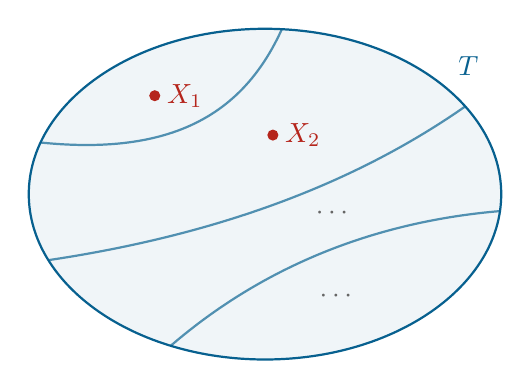
\begin{tikzpicture}
    % (1) Fill of T
    \fill[figBlue!6] (0, 0) ellipse (3.0 and 2.1);

    % (2) Orbit partition curves clipped to T
    \begin{scope}
        \clip (0, 0) ellipse (3.0 and 2.1);
        \draw[thick, figBlue!70] (-3.2, 0.7) .. controls (-1.2, 0.4) and (-0.2, 1.0) .. (0.3, 2.3);
        \draw[thick, figBlue!70] (-3.2, -0.9) .. controls (-0.8, -0.6) and (1.2, 0.1) .. (2.8, 1.3);
        \draw[thick, figBlue!70] (-1.6, -2.3) .. controls (-0.2, -0.9) and (1.5, -0.3) .. (3.2, -0.2);
    \end{scope}

    % (3) Outline of T
    \draw[thick, figBlue] (0, 0) ellipse (3.0 and 2.1);

    % (4) Orbit representatives
    \fill[chalkRed] (-1.4, 1.25) circle (2pt) (0.1, 0.75) circle (2pt);

    % (5) Text last
    \node[anchor=south west, inner sep=0.15cm, figBlue] at (2.30, 1.35) {$T$};
    \node[anchor=west, inner sep=0.15cm, chalkRed] at (-1.4, 1.25) {$X_1$};
    \node[anchor=west, inner sep=0.15cm, chalkRed] at (0.1, 0.75) {$X_2$};
    \node[figGray] at (0.85, -0.25) {$\cdots$};
    \node[figGray] at (0.90, -1.30) {$\cdots$};
\end{tikzpicture}
\end{center}

Since the finite set $T$ is partitioned into finitely many disjoint $G$-orbits, choosing one representative $X_i \in T$ from each orbit gives the orbit decomposition formula:
\begin{equation}\label{eq:orbit-decomposition}
|T| = \sum_{X_i} |\operatorname{Orb}(X_i)|.
\end{equation}
By \eqref{eq:T-cardinality} and \eqref{eq:p-not-div-binom}, the left-hand side satisfies
\[
|T| = \binom{n}{p^k} \quad \text{and} \quad p \nmid |T|.
\]
Therefore, $p$ cannot divide $|\operatorname{Orb}(X_i)|$ for every orbit, so there must exist at least one representative $X_j \in T$ such that
\begin{equation}\label{eq:p-not-div-orb}
p \nmid |\operatorname{Orb}(X_j)|.
\end{equation}

\begin{steps}[Why At Least One Orbit Size Is Coprime to \texorpdfstring{$p$}{p}]
If $p$ divided $|\operatorname{Orb}(X_i)|$ for every orbit in the sum \eqref{eq:orbit-decomposition}, then $p$ would divide the entire sum $|T| = \binom{n}{p^k}$, contradicting $p \nmid |T|$ from \eqref{eq:p-not-div-binom}. Hence, at least one summand $|\operatorname{Orb}(X_j)|$ is not divisible by $p$.
\end{steps}
\end{content}

\begin{speech}[00:13:59 - 00:15:49]
All right, now we use the orbit-stabilizer theorem for that orbit. So, use this orbit-stabilizer theorem \inlinemetanote{writes: Use Orb-Stab Thm}, and what does it say? It says the size of $G$ divided by the size of the stabilizer of that $X_j$ equals the size of this orbit \inlinemetanote{writes: $\frac{|G|}{|\operatorname{Stab}(X_j)|} = |\operatorname{Orb}(X_j)|$}. That's the orbit-stabilizer theorem.

Okay. And what do we know? That this thing here, the size of $G$, is $n$, and $n$ is equal to $p$ to the $k$ times $m$ \inlinemetanote{writes \qt{$p^k m$} with an arrow pointing to $|G|$}, okay? That's what the top is here, right? And this thing has no $p$'s, because $p$ does not divide this \inlinemetanote{writes \qt{has no $p$'s} with an arrow pointing to $|\operatorname{Orb}(X_j)|$}. Okay?

So, where could all the $p$'s go? How can you have this? We've got a lot of $p$'s here, no $p$'s here. How could this happen? All the $p$'s have to be here. They have to kill all the $p$'s. So, the conclusion here is that $p$ to the $k$ divides the stabilizer --- well, the size of the stabilizer \inlinemetanote{writes: $\implies p^k \mid |\operatorname{Stab}(X_j)|$}, because there's conservation of $p$'s, they can't just leave. Okay. And so, is that clear? We got a big number of $p$'s here, $p$ to the $k$. There's no $p$'s here. The only way to get rid of them is if we had divided them out. Okay?
\end{speech}

\begin{content}[Divisibility of \texorpdfstring{$|\operatorname{Stab}(X_j)|$}{|Stab(X\_j)|} by \texorpdfstring{$p^k$}{p\^{}k}]
Applying the Orbit-Stabilizer Theorem to the special representative $X_j \in T$ from \eqref{eq:p-not-div-orb}, we obtain:
\begin{equation}\label{eq:orb-stab-Xj}
\frac{|G|}{|\operatorname{Stab}(X_j)|} = |\operatorname{Orb}(X_j)|.
\end{equation}
Substituting $|G| = n = p^k m$ from \eqref{eq:n-factorization} into \eqref{eq:orb-stab-Xj} and clearing denominators yields
\[
p^k m = |\operatorname{Stab}(X_j)| \cdot |\operatorname{Orb}(X_j)|.
\]
Since $p \nmid |\operatorname{Orb}(X_j)|$ (\qt{$|\operatorname{Orb}(X_j)|$ has no $p$'s}), the prime power $p^k$ is coprime to $|\operatorname{Orb}(X_j)|$, i.e., $\gcd\bigl(p^k, |\operatorname{Orb}(X_j)|\bigr) = 1$. By Euclid's Lemma applied to the factors of $p^k$, all $k$ factors of $p$ on the left-hand side must divide $|\operatorname{Stab}(X_j)|$:
\begin{equation}\label{eq:pk-divides-stab}
\implies p^k \mid |\operatorname{Stab}(X_j)|.
\end{equation}
\end{content}

\begin{insight}[\qt{Conservation of $p$'s} in the Orbit-Stabilizer Identity]
Because $p^k m = |\operatorname{Stab}(X_j)| \cdot |\operatorname{Orb}(X_j)|$ is an equality of positive integers and $|\operatorname{Orb}(X_j)|$ carries zero factors of $p$, unique prime factorization guarantees that every factor of $p$ present in $|G| = p^k m$ must appear in $|\operatorname{Stab}(X_j)|$. Combined with the upper bound $|\operatorname{Stab}(X_j)| \le p^k$, this forces exact equality.
\end{insight}

\begin{speech}[00:15:49 - 00:16:33]
And so, this proves for this special one, for this very special $X_j$, the order of the stabilizer --- I'm never going to do this again --- is at least $p$ to the $k$ \inlinemetanote{writes \qt{for $X_j$} and an aborted chalk mark, then writes: $|\operatorname{Stab}(X_j)| \ge p^k$}. Otherwise, how could it divide it? It's not zero. Okay.

And that's it. That's like an amazingly gorgeous proof. So, we found the group now: it's the stabilizer of this particular one. It has size less than $p$ to the $k$ and greater than $p$ to the $k$, so it has size $p$ to the $k$ and we're done \inlinemetanote{changes $\ge$ to $=$ so it reads $|\operatorname{Stab}(X_j)| = p^k$ and draws a QED box}. So, that is an amazing proof.
\end{speech}

\begin{content}[Conclusion and Complete Proof of \cref{thm:sylow-1}]
Since $|\operatorname{Stab}(X_j)| > 0$ (every stabilizer contains at least the identity element $e \in G$) and $p^k \mid |\operatorname{Stab}(X_j)|$ by \eqref{eq:pk-divides-stab}, it follows that
\begin{equation}\label{eq:stab-lower-bound}
|\operatorname{Stab}(X_j)| \ge p^k.
\end{equation}
Combining \eqref{eq:stab-lower-bound} with the upper bound $|\operatorname{Stab}(X_j)| \le p^k$ from \cref{lem:stab-bound} gives
\begin{equation}\label{eq:stab-exact-order}
|\operatorname{Stab}(X_j)| = p^k.
\end{equation}
Setting $S := \operatorname{Stab}(X_j) \subset G$ therefore produces the required subgroup of $G$ of order $p^k$, completing the proof of \cref{thm:sylow-1}.

\par\vspace{1ex}\noindent
\textbf{Consolidated Proof Summary:}
\par\vspace{0.5ex}\noindent
\textbf{1. Action on $p^k$-Element Subsets:} Let $T := \bigl\{ X \subset G \;\big|\; |X| = p^k \bigr\}$, with $|T| = \binom{n}{p^k}$ and $p \nmid |T|$ by \eqref{eq:p-not-div-binom}. The group $G$ acts on $T$ on the left via $g \cdot X = \{ga \mid a \in X\}$.

\textbf{2. Upper Bound on Stabilizers (\cref{lem:stab-bound}):} For any $X \in T$, fix $a_1 \in X$. The map $\operatorname{Stab}(X) \to X$, $g \mapsto g \cdot a_1$, is injective by group cancellation in $G$, whence $|\operatorname{Stab}(X)| \le |X| = p^k$.

\textbf{3. Finding an Orbit Coprime to $p$:} Decomposing $T$ into $G$-orbits yields $|T| = \sum_{X_i} |\operatorname{Orb}(X_i)|$. Since $p \nmid |T|$, there exists $X_j \in T$ with $p \nmid |\operatorname{Orb}(X_j)|$.

\textbf{4. Orbit-Stabilizer Squeeze:} By the Orbit-Stabilizer Theorem, $p^k m = |G| = |\operatorname{Stab}(X_j)| \cdot |\operatorname{Orb}(X_j)|$. Since $p \nmid |\operatorname{Orb}(X_j)|$, we obtain $p^k \mid |\operatorname{Stab}(X_j)|$, and hence $|\operatorname{Stab}(X_j)| \ge p^k$. Together with $|\operatorname{Stab}(X_j)| \le p^k$, we conclude $|\operatorname{Stab}(X_j)| = p^k$, so $S := \operatorname{Stab}(X_j)$ is a subgroup of order $p^k$.
\end{content}

\end{proofWrapper}

\begin{speech}[00:16:44 - 00:17:02]
So, this is a proof that shows the power of thinking about these group actions, but it's a really amazing proof.

Okay, that's Sylow $1$, that we have one of the subgroups now.
\end{speech}

\section{Sylow's Second Theorem}

\subsection{Statement and \texorpdfstring{$p$}{p}-Sylow Subgroups}

\begin{speech}[00:17:03 - 00:18:39]
Okay, so Sylow $2$ says something else. So, we're going to head to Sylow $2$ \inlinemetanote{writes \qt{Sylow II} on the lower-left board}.

It's the same hypotheses, I don't write them again: we have $G$, $G$ is a group of order $n$, and we have $p$ to the $k$ is the biggest power of $p$ that divides that. Well, maybe I write it anyway \inlinemetanote{writes: $|G| = n = p^k m$, $p \nmid m$}, so we don't get confused.

So, let $H$ be any subgroup of order $p$ to the $\ell$ \inlinemetanote{writes: Let $H \subset G$ be any subgroup of order $p^\ell$}, okay? We just take any subgroup of order $p$ to the $\ell$. Of course, in this case $\ell$ has to be less than or equal to $k$ by Lagrange \inlinemetanote{writes: ($\ell \le k$ by Lagrange)}. Because a subgroup has to have an order which divides, so $\ell$ is... So, we take any one.

Then Sylow $2$ says that $H$ lies in a subgroup $S$ --- let me write it as \qt{there exists} --- there exists $S$ in $G$ \inlinemetanote{begins writing $H \subset$, erases it, and writes: $\exists\, S \subset G$} such that $H$ is in $S$ and the order of $S$ is $p$ to the $k$ \inlinemetanote{writes \qt{such that $H \subset S$} and \qt{$|S| = p^k$}}. So, this says that if you take any subgroup of order $p$ to the $\ell$, actually it sits inside one of our subgroups of order $p$ to the $k$.
\end{speech}

\begin{content}
\begin{theorem}[Sylow's Second Theorem (Sylow 2)]\label[theorem]{thm:sylow-2}
Let $G$ be a finite group of order $|G| = n = p^k m$ with $p \nmid m$ (where $p$ is prime and $k \ge 0$). Let $H \subset G$ be any subgroup of order $|H| = p^\ell$ (so $\ell \le k$ by Lagrange's Theorem). Then there exists a subgroup $S \subset G$ such that
\[
H \subset S \quad \text{and} \quad |S| = p^k.
\]
\end{theorem}

\begin{steps}[Why Lagrange's Theorem Forces \texorpdfstring{$\ell \le k$}{l <= k}]
By Lagrange's Theorem, the order $|H| = p^\ell$ divides $|G| = p^k m$. Since $p$ is prime and $p \nmid m$, the exponent of $p$ in $|H|$ cannot exceed the exponent $k$ of $p$ in $|G|$, giving $\ell \le k$.
\end{steps}
\end{content}

\begin{hidden}
% timestamp: 00:05:49
% topic: Completed proof of Sylow 1 and stated Sylow 2
% board_state: thm:sylow-1, thm:sylow-2
% next_goal: Define p-Sylow subgroups, restate Sylow 2, and begin the proof of Sylow 2.
% open_loops: none
\end{hidden}

\begin{speech}[00:18:39 - 00:19:58]
So, the terminology for this, by the way, is that for $G$, if $S$ is a subgroup of $G$, where $S$ is of order $p$ to the $k$, then --- this is the definition --- $S$ is called a \newterm{$p$-Sylow subgroup} \inlinemetanote{writes \qt{$G$}, \qt{if $S \subset G \quad |S| = p^k$}, and boxes \qt{$S$ is called a $p$-Sylow subgroup}}.

If you have a finite group, and you take this maximal power of $p$, if you ever find a subgroup of that order, it's called a $p$-Sylow subgroup. Sylow $1$ says there exist $p$-Sylow subgroups \inlinemetanote{points up to Sylow 1, then back down}. Sylow $2$ says that if I take any subgroup of order $p$ to the $\ell$, it actually sits inside a $p$-Sylow subgroup. Okay?

So, maybe I write that in words: Sylow $2$ says that every subgroup $H$ in $G$, where $H$ has some power of $p$ order, $H$ sits in a $p$-Sylow subgroup \inlinemetanote{writes: Sylow 2: every subgp $H \subset G$ w/ $|H| = p^\ell$, $H$ sits in a $p$-Sylow subgp.}. I'm just saying over what I've said already. So, we have to prove it.
\end{speech}

\begin{content}
\begin{definition}[\texorpdfstring{$p$}{p}-Sylow Subgroup]\label[definition]{def:p-sylow-subgroup}
Let $G$ be a finite group of order $|G| = n = p^k m$ with $p \nmid m$. If $S \subset G$ is a subgroup with $|S| = p^k$, then
\begin{center}
\fbox{$S$ is called a \newterm{$p$-Sylow subgroup}.}
\end{center}
\end{definition}

\begin{remark}[Restatement of Sylow 2 in Terms of \texorpdfstring{$p$}{p}-Sylow Subgroups]\label[remark]{rem:sylow-2-restatement}
In this terminology, \cref{thm:sylow-1} (Sylow 1) guarantees the existence of at least one $p$-Sylow subgroup of $G$, and \cref{thm:sylow-2} (Sylow 2) states that every subgroup $H \subset G$ with $|H| = p^\ell$ is contained in a $p$-Sylow subgroup of $G$.
\end{remark}
\end{content}

\begin{aiNote}[Beyond the Lecture: Textbook Conventions for Sylow's Theorems]
% [PERSISTENT, ADDITION]
Textbooks differ in how they label Sylow's theorems: many sources formulate Sylow's Second Theorem as the statement that any two $p$-Sylow subgroups of $G$ are conjugate (or combine that conjugacy statement with the containment of every $p$-subgroup $H$ in a conjugate $x P x^{-1}$ of a fixed $p$-Sylow subgroup $P$). This lecture presents the containment property of every $p$-power-order subgroup inside a $p$-Sylow subgroup as Sylow 2.
\end{aiNote}

\begin{proofWrapper}[Proof of \cref{thm:sylow-2}]

\subsection{Fixing a \texorpdfstring{$p$}{p}-Sylow Subgroup and Initial Reduction}

\begin{speech}[00:19:58 - 00:21:07]
All right, so we have to name one, so let's call it $P$. So, I'm going to give the proof now \inlinemetanote{writes: Proof}. So, let $P$ in $G$ be a $p$-Sylow subgroup \inlinemetanote{writes: Let $P \subset G$ be a $p$-Sylow subgp.}. The size of this is $p$ to the $k$ \inlinemetanote{writes: $|P| = p^k$}. It's capital $P$. So, this exists by Sylow $1$ \inlinemetanote{writes: (Sylow I)}. All right?

And now we have $H$: we are given the subgroup $H$ in $G$, where the order of $H$ is $p$ to the $\ell$ \inlinemetanote{writes \qt{We are given} and \qt{$H \subset G \quad |H| = p^\ell$}}. And first of all, we can just assume $\ell$ is positive, because if we were given a subgroup of order $p$ to the zero, that subgroup is order $1$, which means it's only the neutral element, and the neutral element sits inside here (i.e., $P$), so we don't have to confuse ourselves with this case \inlinemetanote{writes: $\ell > 0$}. So, we can assume that $\ell$ is positive.

Okay, and we're going to use a group action, of course.
\end{speech}

\begin{content}[Choice of \texorpdfstring{$P$}{P} and Reduction to \texorpdfstring{$\ell > 0$}{l > 0}]
By \cref{thm:sylow-1} (Sylow 1), there exists at least one $p$-Sylow subgroup $P \subset G$, so that
\[
|P| = p^k.
\]
We are given an arbitrary subgroup $H \subset G$ of order $|H| = p^\ell$. We may assume without loss of generality that
\[
\ell > 0,
\]
because if $\ell = 0$, then $|H| = p^0 = 1$, which means $H = \{e\}$ consists solely of the neutral element $e \in G$, and clearly $\{e\} \subset P$.
\end{content}

\subsection{Action of \texorpdfstring{$H$}{H} on the Left Coset Space \texorpdfstring{$\faktor{G}{P}$}{G/P}}

\begin{speech}[00:21:13 - 00:22:44]
So, the question is, which group action do we use for this? \inlinemetanote{erases the lower-left panel}

We have $G$, and our $p$-Sylow subgroup $P$ \inlinemetanote{writes: $P \subset G$}. So, we can consider this coset space: this is the set of left cosets \inlinemetanote{writes \qt{$\faktor{G}{P}$} with an arrow from \qt{set of left cosets} pointing to it}. And we have seen that $G$ acts on this \inlinemetanote{writes: $G \curvearrowright \faktor{G}{P}$}. That's the standard action on left cosets \inlinemetanote{writes \qt{standard action on left cosets} with an arrow pointing to $\curvearrowright$}. We discussed this yesterday.

Okay, but that's not $H$, there's no $H$ there. But we can always act by a subgroup here. So, we take this as the standard action \inlinemetanote{writes: $G \times \faktor{G}{P} \to \faktor{G}{P}$}. And we can just restrict this to be inside $H$. So, we get $H$ cross $G$ mod $P$ to $G$ mod $P$ \inlinemetanote{writes \qt{$H \times \faktor{G}{P} \to \faktor{G}{P}$} below \qt{$G \times \faktor{G}{P} \to \faktor{G}{P}$} with an inclusion mark from $H$ up to $G$}. Okay? So, this is the action we're going to take.

Is this restriction clear? We already know how $G$ acts on left cosets. $H$ is a subgroup, so it just acts as if it were an element of $G$. Okay, so this is the action we'll consider: we consider this action in the proof \inlinemetanote{writes \qt{We consider this action} pointing to $H \times \faktor{G}{P} \to \faktor{G}{P}$}.
\end{speech}

\begin{content}[Restricting the Left Coset Action to \texorpdfstring{$H$}{H}]
Let $P \subset G$ be the fixed $p$-Sylow subgroup, and consider the set of left cosets of $P$ in $G$, denoted by $\faktor{G}{P}$. The group $G$ acts on $\faktor{G}{P}$ via the standard left-multiplication action on left cosets:
\begin{align*}
G \curvearrowright \faktor{G}{P}, \qquad G \times \faktor{G}{P} &\to \faktor{G}{P} \\
(g, xP) &\mapsto (gx)P.
\end{align*}
Since $H \subset G$ is a subgroup, we restrict this standard action from $G$ to $H$ to obtain the action that we consider in the proof:
\begin{align*}
H \times \faktor{G}{P} &\to \faktor{G}{P} \\
(h, xP) &\mapsto (hx)P.
\end{align*}

\begin{steps}[Why Restricting a Group Action to a Subgroup Always Works]
If $G \times S \to S$ satisfies the identity axiom ($e \cdot s = s$) and compatibility ($g_1 \cdot (g_2 \cdot s) = (g_1 g_2) \cdot s$) for all $g_1, g_2 \in G$, then the exact same axioms hold automatically when $g_1, g_2$ are restricted to elements of any subgroup $H \subset G$ (since $e \in H$ and $H$ is closed under multiplication).
\end{steps}
\end{content}

\begin{speech}[00:22:46 - 00:23:47]
I'll try to make big $P$'s here so you don't get confused. What are we going to do with this action? Well, we'd like to know what is the size of this set \inlinemetanote{writes: $\bigl|\faktor{G}{P}\bigr| =$}. And the answer is that we know this is $n$, and this is $p$ to the $k$, and so this is $m$ \inlinemetanote{writes: $\frac{n}{p^k} = m$}, because Lagrange says that the size of this is equal to the size of $G$... size of $P$ \inlinemetanote{writes \qt{$\frac{|G|}{|P|}$} below $\bigl|\faktor{G}{P}\bigr|$}. Okay? So, that's $m$.

And we know one thing about $m$: $p$ does not divide $m$ \inlinemetanote{writes: $p \nmid m$}. All right? So, this means we have $H$ acting on this $G$ mod $P$ \inlinemetanote{writes: $H \curvearrowright \faktor{G}{P}$}. And the size of this set here is not divisible by $p$ \inlinemetanote{writes: $\bigl|\faktor{G}{P}\bigr|$ is not div. by $p$}.
\end{speech}

\begin{content}[Cardinality of the Coset Space \texorpdfstring{$\faktor{G}{P}$}{G/P}]
By Lagrange's Theorem, the number of left cosets of $P$ in $G$ is
\begin{equation}\label{eq:coset-space-size}
\left|\faktor{G}{P}\right| = \frac{|G|}{|P|} = \frac{n}{p^k} = m.
\end{equation}
Since $p \nmid m$, we have an action $H \curvearrowright \faktor{G}{P}$ on a finite set whose cardinality $\bigl|\faktor{G}{P}\bigr|$ is not divisible by $p$ (i.e., $p \nmid \bigl|\faktor{G}{P}\bigr|$).
\end{content}

\subsection{Existence of an \texorpdfstring{$H$}{H}-Fixed Point in \texorpdfstring{$\faktor{G}{P}$}{G/P}}

\begin{speech}[00:23:48 - 00:25:39]
All right. So, the conclusion --- and we've seen this kind of argument before --- the conclusion we will see is that there must be a fixed point, an $H$-fixed point in $G$ mod $P$ \inlinemetanote{writes: Conclusion is that there must be an $H$-fixed pt in $\faktor{G}{P}$}. All right? I'll give you an argument for this, but it should not be a surprise.

Well, I'll say it in words and I'll write it down clear. So, because we can divide this (i.e., $\faktor{G}{P}$) in terms of the orbits \inlinemetanote{points at $\faktor{G}{P}$}, right? And the orbits always have orders that are divisible by the order of $H$ (i.e., divide the order of $H$). That's by the orbit-stabilizer theorem. This (i.e., $|H|$) is a power of $p$, so the only possibility for the orbits are powers of $p$.

If all the orbits took positive powers of $p$, then this (i.e., $\bigl|\faktor{G}{P}\bigr|$) would be divisible by $p$, but it's not divisible by $p$. So, there must be one orbit that takes the only power of $p$ that's not divisible by $p$, which is $p$ to the zero, and that would be a fixed point. That's the argument in words. We can write it, but we've done this argument before.

What's important in this argument is the size of $H$ is a power of $p$, and the size of the set does not divide $p$... $p$ is not divisible by that, sorry... $p$ does not divide the size of the set \inlinemetanote{erases the lower-right panel while speaking}. So, let's try to write it out somehow longhand.
\end{speech}

\begin{content}[Fixed-Point Claim for \texorpdfstring{$H \curvearrowright \faktor{G}{P}$}{H acting on G/P}]
\begin{claim}[Existence of an $H$-Fixed Point in \texorpdfstring{$\faktor{G}{P}$}{G/P}]\label[claim]{clm:h-fixed-point}
For the restricted action $H \curvearrowright \faktor{G}{P}$, since $|H| = p^\ell$ is a power of $p$ and $p \nmid \bigl|\faktor{G}{P}\bigr|$, there must exist an $H$-fixed point in $\faktor{G}{P}$.
\end{claim}
\end{content}

\begin{aiNote}[Verbal Slip: \qt{divisible by} vs. \qt{divide}]
% [PERSISTENT]
At 00:24:28, the lecturer briefly misspeaks by saying that the orbits have \qt{orders that are divisible by the order of $H$} instead of saying that the orbit sizes \emph{divide} $|H|$. By the Orbit-Stabilizer Theorem ($|\operatorname{Orb}(z_i)| = \frac{|H|}{|\operatorname{Stab}(z_i)|}$), each orbit size divides $|H| = p^\ell$, which is what the lecturer immediately uses to deduce that every orbit size is a power of $p$ and writes explicitly in the derivation below.
\end{aiNote}

\begin{hidden}
% timestamp: 00:12:49
% topic: Restricted action H on G/P and fixed-point claim
% board_state: thm:sylow-2, def:p-sylow-subgroup, eq:coset-space-size, clm:h-fixed-point
% next_goal: Write out the orbit-decomposition proof of Claim clm:h-fixed-point and analyze the resulting fixed-point coset equation hxP = xP.
% open_loops: none
\end{hidden}

\begin{speech}[00:25:40 - 00:27:50]
So, the picture that we've drawn many times now: here's $H$ acting on this set \inlinemetanote{writes \qt{$H \curvearrowright$} and draws a partitioned loop labeled $\faktor{G}{P}$}. This is cosets here, so this breaks up into the orbit spaces. Okay?

And the orbit-stabilizer theorem says --- I mean, sorry --- the size here, this is equal to $m$, is equal to the sum of all the orbits \inlinemetanote{writes: $m = \bigl|\faktor{G}{P}\bigr| = \sum |\operatorname{Orb}(z_i)|$}. It's the same thing we always write. So, maybe I put $z_i$ here \inlinemetanote{writes \qt{$z_i$} beneath $\sum$}. We have some $z_1$ here, and $z_2$ here, and so on \inlinemetanote{draws dots labeled $z_1$ and $z_2$ inside two regions of $\faktor{G}{P}$}. Okay? This is what we always write.

Now, the orbit-stabilizer theorem says that the size of this orbit is equal to the size of $H$ divided by the size of the stabilizer \inlinemetanote{writes: $|\operatorname{Orb}(z_i)| = \frac{|H|}{|\operatorname{Stab}(z_i)|}$}. Okay? This thing, $H$, upstairs is a power of $p$. That's all it is, there's nothing else \inlinemetanote{writes \qt{$p^\ell$} with an arrow from $|H|$}. The order of $H$ is a power of $p$: that was the assumption. So, the only possibilities for this orbit are powers of $p$. That's it.

But it cannot be that every orbit is a positive power of $p$, because then this thing (i.e., $m$) would be divisible by $p$, and it's not divisible by $p$, because $m$ is not divisible by $p$ \inlinemetanote{points at the sum and back to $m$}. So, there must be one orbit whose size is not a positive power of $p$. It has to be a power of $p$, but not a positive power of $p$. So, the only possibility is $p$ to the zero, and that orbit is a fixed point.

So, there exists $z_i$ such that orbit $z_i$ is equal to $p$ to the zero \inlinemetanote{writes: $\exists\, z_i \text{ s.t. } |\operatorname{Orb}(z_i)| = p^0$}. And then $z_i$ is an $H$-fixed point \inlinemetanote{writes: then $z_i$ is $H$-fixed pt.}, because it means that the stabilizer takes up all of $H$ and it's a fixed point.
\end{speech}

\begin{content}[Orbit Decomposition Proof of \cref{clm:h-fixed-point}]
\definecolor{figBlue}{HTML}{07608F} % RGB (7, 96, 143): petrol blue (MidnightBlue)
\definecolor{chalkRed}{HTML}{B5251C} % RGB (181, 37, 28): brick red (BrickRed)
\definecolor{figGray}{HTML}{666666} % RGB (102, 102, 102): dark gray
\begin{hidden}
- Canvas: no scale, coordinates in cm; x in [-2.2, 4.5], y in [-2.0, 2.2]
- Order: (1) light fill of G/P; (2) orbit partition curves clipped to G/P; (3) outline of G/P; (4) action arrow from H;
  (5) representative dots z_1, z_2; (6) all text last
- Coordinates:
  G/P: ellipse centre (1.5, 0), radii 2.2 and 1.9 (x in [-0.7, 3.7], y in [-1.9, 1.9]).
  Curve 1 (left vertical divider): plot[domain=-1.9:1.9, samples=30] ({0.2 + 0.08*\x*\x}, \x);
  passes exactly through (0.22, 0.5) and (0.22, -0.5).
  Curve 2 (upper-right divider): (0.22, 0.5) .. controls (1.2, 0.85) and (2.4, 0.45) .. (3.8, 0.75), mid y ~ 0.64.
  Curve 3 (lower-right divider): (0.22, -0.5) .. controls (1.2, -0.25) and (2.4, -0.65) .. (3.8, -0.45), mid y ~ -0.46.
  Representatives:
  z_1 = (1.65, 1.05): in ellipse ((0.15/2.2)^2 + (1.05/1.9)^2 = 0.005 + 0.305 = 0.310 < 1);
  0.41 above Curve 2 (~0.64) and 0.84 below ellipse top (1.895).
  z_2 = (1.65, -0.05): 0.69 below Curve 2 and 0.41 above Curve 3 (~-0.46).
  H and action arrow: H node centred at (-1.6, 1.35); arrow from (-1.3, 1.45) to[bend left=25] (-0.35, 1.25)
  (at y = 1.25, ellipse left edge is 1.5 - 2.2 * 0.753 = -0.16, so tip stops 0.19 left of ellipse).
- Labels (attached, inner sep=0.15cm):
  "H" at (-1.6, 1.35);
  "\faktor{G}{P}" at ellipse boundary (1.5 + 2.2 cos 35, 1.9 sin 35) = (3.30, 1.09), anchor=south west;
  "z_1" anchor=south at (1.65, 1.05), inner sep=0.12cm;
  "z_2" anchor=south at (1.65, -0.05), inner sep=0.12cm.
- Collisions: z_1 label ends around y = 1.57, 0.32 below top outline; z_2 label ends around y = 0.47, 0.17 below Curve 2;
  G/P label grows outside ellipse to upper-right; H and its curved arrow stay well left of ellipse.
\end{hidden}
\begin{center}
\begin{tikzpicture}[>=Stealth]
    % (1) Fill of G/P
    \fill[figBlue!6] (1.5, 0) ellipse (2.2 and 1.9);

    % (2) Orbit partition curves clipped to G/P
    \begin{scope}
        \clip (1.5, 0) ellipse (2.2 and 1.9);
        \draw[thick, figBlue!70] plot[domain=-1.9:1.9, samples=30] ({0.2 + 0.08*\x*\x}, \x);
        \draw[thick, figBlue!70] (0.22, 0.5) .. controls (1.2, 0.85) and (2.4, 0.45) .. (3.8, 0.75);
        \draw[thick, figBlue!70] (0.22, -0.5) .. controls (1.2, -0.25) and (2.4, -0.65) .. (3.8, -0.45);
    \end{scope}

    % (3) Outline of G/P
    \draw[thick, figBlue] (1.5, 0) ellipse (2.2 and 1.9);

    % (4) Action arrow from H
    \draw[->, thick] (-1.3, 1.45) to[bend left=25] (-0.35, 1.25);

    % (5) Orbit representatives
    \fill[chalkRed] (1.65, 1.05) circle (2pt) (1.65, -0.05) circle (2pt);

    % (6) Text last
    \node[inner sep=0.15cm] at (-1.6, 1.35) {$H$};
    \node[anchor=south west, inner sep=0.15cm, figBlue] at (3.30, 1.09) {$\faktor{G}{P}$};
    \node[anchor=south, inner sep=0.12cm, chalkRed] at (1.65, 1.05) {$z_1$};
    \node[anchor=south, inner sep=0.12cm, chalkRed] at (1.65, -0.05) {$z_2$};
\end{tikzpicture}
\end{center}

\begin{proof}[Proof of \cref{clm:h-fixed-point}]
Decomposing the finite set $\faktor{G}{P}$ into its $H$-orbits with representatives $z_1, z_2, \dots \in \faktor{G}{P}$ gives
\begin{equation}\label{eq:gp-orbit-decomp}
m = \left|\faktor{G}{P}\right| = \sum_{z_i} |\operatorname{Orb}(z_i)|.
\end{equation}
For each representative $z_i$, the Orbit-Stabilizer Theorem for the action $H \curvearrowright \faktor{G}{P}$ gives
\begin{equation}\label{eq:h-orb-stab}
|\operatorname{Orb}(z_i)| = \frac{|H|}{|\operatorname{Stab}(z_i)|},
\end{equation}
where $\operatorname{Stab}(z_i) := \{ h \in H \mid h \cdot z_i = z_i \}$ denotes the stabilizer of $z_i$ in $H$. Since $|H| = p^\ell$, the integer $|\operatorname{Orb}(z_i)|$ divides $p^\ell$, so the only possible values for $|\operatorname{Orb}(z_i)|$ are powers of $p$ (namely $p^0, p^1, \dots, p^\ell$).

Now suppose for contradiction that every orbit had size equal to a positive power of $p$. Then every summand on the right-hand side of \eqref{eq:gp-orbit-decomp} would be divisible by $p$, which would imply $p \mid m$, contradicting $p \nmid m$. Therefore, there must exist at least one representative $z_i \in \faktor{G}{P}$ whose orbit size is not a positive power of $p$. The only remaining power of $p$ is $p^0$:
\begin{equation}\label{eq:fixed-point-orbit}
\exists\, z_i \in \faktor{G}{P} \text{ such that } |\operatorname{Orb}(z_i)| = p^0 = 1.
\end{equation}
By \eqref{eq:h-orb-stab}, $|\operatorname{Orb}(z_i)| = 1$ means $|\operatorname{Stab}(z_i)| = |H|$, so $\operatorname{Stab}(z_i) = H$. Hence, $z_i$ is an $H$-fixed point in $\faktor{G}{P}$.
\end{proof}

\begin{steps}[Singleton Orbits as Fixed Points]
In the orbit partition diagram of $\faktor{G}{P}$ above, the orbit of $z_i$ from \eqref{eq:fixed-point-orbit} has cardinality $p^0 = 1$, meaning it is a single-element cell $\{z_i\}$ that every element $h \in H$ maps back to itself.
\end{steps}
\end{content}

\subsection{Interpreting the Fixed-Point Equation}

\begin{speech}[00:27:50 - 00:29:14]
All right, so we found one $z_i$. So, this $z_i$ --- this one that's a fixed point --- is an element of this \inlinemetanote{writes: $z_i \in \faktor{G}{P}$}, right? It's a coset space, so we can write $z_i$ as some $x P$ \inlinemetanote{writes: $z_i = x P$}. That's the left coset of $x$, where $x$ is in $G$ \inlinemetanote{writes: $x \in G$}. So, the $z_i$ is an element of this coset space, and now I'm just writing explicitly it's a coset.

And what we know about this is it's a fixed point. That means we know, since it's an $H$-fixed point --- I don't have to say $H$-fixed, I could just say fixed for the action we're considering, but since there are $G$'s and $H$'s, I'm just being very specific and saying $H$-fixed point --- we know that if I take any element in $H$, if I take $h x$, this coset (i.e., $h x P$), it has to be just this coset (i.e., $x P$) \inlinemetanote{writes: We know ($H$-fixed pt.) $\forall\, h \quad h x P = x P$}. Okay? That's what it means, for any $h$.

All right, so we're going to look at this equation. What does it say?

But the whole point of this analysis of this action of $H$ on the left coset space was to find this fixed point. That was the whole purpose of that analysis. Well, we found it now, and that fixed point has this property \inlinemetanote{points at $\forall\, h \quad h x P = x P$}.
\end{speech}

\begin{content}[Explicit Coset Form of the \texorpdfstring{$H$}{H}-Fixed Point]
Since $z_i \in \faktor{G}{P}$ is an element of the left coset space, we can write it explicitly as
\[
z_i = x P \quad \text{for some } x \in G.
\]
The fact that $z_i$ is an $H$-fixed point under the restricted left-multiplication action means that every element of $H$ leaves the coset $x P$ invariant:
\begin{equation}\label{eq:fixed-point-coset}
\forall\, h \in H \colon \quad h x P = x P.
\end{equation}
\end{content}

\begin{speech}[00:29:24 - 00:30:35]
So, let's try to think about that, this fixed point equation. So, we remember here that $P$ inside $G$ to start, this was a $p$-Sylow subgroup \inlinemetanote{writes: $P \subset G$ is $p$-Sylow subgroup}. So, in particular, the order of this is $p$ to the $k$ \inlinemetanote{writes: $|P| = p^k$}. And now we have the fixed point equation \inlinemetanote{writes: Fixed point equation}.

The fixed point equation says that --- I just repeat it --- for every $h$, if I take $h$ times this coset, I get back this coset \inlinemetanote{writes: $\forall\, h \in H \quad h x P = x P$}. All right, so here is this \inlinemetanote{writes: $x P \in \faktor{G}{P}$ is $H$-fixed}.

So, this is the summary from the previous part. We start with this $p$-Sylow subgroup. It has the right order for the maximal power of $p$. There's the $H$-action: by our analysis of this orbit-stabilizer theorem, there is some coset here which is $H$-fixed. This is the $H$-fixed equation, that's for every $h$. Oh, it's already written there. Okay.
\end{speech}

\begin{content}[Summary of Setup and Fixed-Point Equation]
Summarizing the ingredients obtained so far:
\begin{itemize}
    \item $P \subset G$ is a $p$-Sylow subgroup, so its order is $|P| = p^k$.
    \item By our orbit-stabilizer analysis, there exists an $H$-fixed left coset $x P \in \faktor{G}{P}$, which satisfies the \newterm{fixed-point equation}:
    \begin{equation}\label{eq:fixed-point-equation-s2}
    \forall\, h \in H \colon \quad h x P = x P.
    \end{equation}
\end{itemize}
\end{content}

\begin{speech}[00:30:35 - 00:32:09]
So, we need to think a little bit about what this means. So, in this coset, this is $h x$ \inlinemetanote{writes: $h x P$}... So, when I write this, I hope you understand what this coset is, you know: $x$ is an element of $G$ \inlinemetanote{writes: $x \in G$}. $h$ is an element of $H$ inside $G$ \inlinemetanote{writes: $h \in H \subset G$}, so when I multiply $h$ times $x$, that's inside $G$ \inlinemetanote{writes: $h x \in G$}, and this is the coset \inlinemetanote{points at $h x P$}. All right?

In particular, $h x$ is in this coset \inlinemetanote{writes: $h x P \ni h x$}, because this $P$ could be put $1$ there. But it better be also in this coset, so that means $h x$ must also be here in $x P$ \inlinemetanote{writes: $h x$ must also be in $x P$}.

So, what does that mean? That means that there must be some element $z$ in $P$ such that $h x$ equals $x z$ \inlinemetanote{writes \qt{$\exists\, z \in P$ such that $h x = x z$} with an arrow from $z$ pointing down to $P$}, where this (i.e., $z$) is an element of $P$, this (i.e., $x$) is an element of $G$, this (i.e., $x$) is an element of $G$. That's the fixed one. We're not ever moving $x$. $x$ is already chosen here \inlinemetanote{points at $x P \in \faktor{G}{P}$}.

These are some fixed... maybe I should erase it because you remember it. $x$ is fixed, we start with $h$, $x$ is fixed, and it's saying we can always solve this equation. I mean, we found our $x$, and it says that for every $h$, we can solve this equation, that $h x$ equals $x$ times something in $P$ --- we can always solve it. That's what it says.
\end{speech}

\begin{content}[Elementwise Membership and Existence of \texorpdfstring{$z \in P$}{z in P}]
Fix an arbitrary element $h \in H \subset G$. Since $x \in G$, the product $h x \in G$ is an element of $G$, and $h x P$ is the left coset of $P$ represented by $h x$.

Because $P$ is a subgroup, it contains the identity element $1 \in P$ (or $e \in P$), and therefore:
\[
h x P \ni h x.
\]
By the fixed-point equation \eqref{eq:fixed-point-equation-s2}, we have $h x P = x P$, so $h x$ must also belong to $x P$ ($h x \in x P$). By the definition of the left coset $x P = \{ x z \mid z \in P \}$, this implies:
\begin{equation}\label{eq:hx-equals-xz}
\exists\, z \in P \text{ such that } h x = x z.
\end{equation}

\begin{steps}[Keeping Track of Fixed vs. Quantified Variables]
Notice the order of quantifiers in \eqref{eq:hx-equals-xz}: the element $x \in G$ was fixed once and for all by choosing the $H$-fixed coset $x P \in \faktor{G}{P}$. Then, for each $h \in H$, there exists an element $z \in P$ (which depends on $h$) satisfying $h x = x z$.
\end{steps}
\end{content}

\begin{hidden}
% timestamp: 00:06:29
% topic: Fixed-point coset equation analysis in the proof of Sylow 2
% board_state: thm:sylow-2, eq:fixed-point-equation-s2, eq:hx-equals-xz
% next_goal: Solve hx = xz for h to conclude H \subset x P x^{-1}, verify x P x^{-1} is a p-Sylow subgroup, and move to Sylow 3.
% open_loops: none
\end{hidden}

\begin{speech}[00:32:09 - 00:33:28]
So, what does that mean? That means that actually $h$ is equal to $x z x$ inverse \inlinemetanote{writes: $h = x z x^{-1}$}. And if I rewrite this, this means that $h$ is in the conjugation of $P$ \inlinemetanote{writes: $h \in x P x^{-1}$}.

Remember conjugation: conjugation is a group automorphism. So, if $P$ is a subgroup of $G$ \inlinemetanote{writes: $P \subset G$}, then $x P x$ inverse is also a subgroup of $G$ \inlinemetanote{writes: $x P x^{-1}$}. Maybe it's a different subgroup, maybe not, but anyway it's a subgroup of $G$.

And it's also a $p$-Sylow subgroup. The order of this is the same as the order of $P$ \inlinemetanote{writes: $|x P x^{-1}| = |P|$}, because conjugation is a bijective operation. And the order is $p$ to the $k$ \inlinemetanote{writes: $= p^k$}.

And this is for any $h$: that means $h$ is inside $x P x$ inverse... Wait, that means $H$ is inside $x P x$ inverse \inlinemetanote{writes: $H \subset x P x^{-1}$}, and then we're done \inlinemetanote{draws a QED box}. Because this is a conjugate of the subgroup $P$ that we started with, such a conjugate has the same order as $P$. So, in particular, the conjugate's also a $p$-Sylow subgroup, and we were trying to find a $p$-Sylow subgroup that contains $H$, and we found it. So, that's the end of the proof.
\end{speech}

\begin{content}[Conjugate Containment and Conclusion of Sylow 2]
Multiplying \eqref{eq:hx-equals-xz} on the right by $x^{-1} \in G$ yields
\[
h = x z x^{-1}.
\]
Since $z \in P$, it follows that $h$ lies in the conjugate set $x P x^{-1} := \{ x p x^{-1} \mid p \in P \}$:
\[
h \in x P x^{-1}.
\]
Moreover, conjugation by $x \in G$,
\[
c_x \colon G \to G, \qquad g \mapsto x g x^{-1},
\]
is a group automorphism (in particular, a bijection). Since $P \subset G$ is a subgroup, its image $x P x^{-1} = c_x(P)$ is also a subgroup of $G$, and by bijectivity it has the exact same cardinality:
\[
|x P x^{-1}| = |P| = p^k.
\]
Hence, $S := x P x^{-1}$ is a $p$-Sylow subgroup of $G$. Since $h \in x P x^{-1}$ holds for every $h \in H$, we conclude that
\[
H \subset x P x^{-1}.
\]
Setting $S := x P x^{-1}$ gives a $p$-Sylow subgroup of $G$ containing $H$, completing the proof of \cref{thm:sylow-2}.

\begin{steps}[Why Conjugation Preserves Subgroup Structure and Order]
For any fixed $x \in G$, the map $c_x(g) = x g x^{-1}$ satisfies $c_x(g_1 g_2) = x g_1 g_2 x^{-1} = (x g_1 x^{-1})(x g_2 x^{-1}) = c_x(g_1) c_x(g_2)$ and has two-sided inverse $c_{x^{-1}}$. Because a group automorphism sends subgroups to subgroups of the same order, $x P x^{-1}$ is a subgroup of order $|P| = p^k$.
\end{steps}
\end{content}
\end{proofWrapper}

\begin{speech}[00:33:28 - 00:35:20]
So, in some sense, in this Sylow argument, we've used two different actions. In the first action, we had to find this particular $X_i$ \inlinemetanote{gestures toward the first proof} such that its orbit was not divisible by $p$, and that produced us the $p$-Sylow subgroup.

In the second part, we start with $H$ \inlinemetanote{points at $H$ on the upper-left board}, and we need to find some way to conjugate our given $p$-Sylow subgroup \inlinemetanote{points at $P \subset G$ and $|P| = p^k$} such that $H$ sits in it. And the search for that conjugation turns out to be a search for this fixed point \inlinemetanote{points at $x P \in \faktor{G}{P}$ is $H$-fixed}, and the fixed point exists again for these arithmetic reasons.

These are really great arguments, and they're not obvious arguments at all. It's not like the connection of the definitions to the results. They are real ideas in these arguments, which are really pretty cool ideas.

So, usually when there's an argument with an actual idea, it means you don't fully understand it the first time you see it. You have to think about it. But these... these are really incredibly cool arguments.

That's Sylow $2$. Sylow $1$ says the existence of a $p$-Sylow subgroup, Sylow $2$ says that any subgroup of order $p$ to the $\ell$ sits inside a $p$-Sylow subgroup, and there's Sylow $3$.

Sylow $3$ says that all $p$-Sylow subgroups are conjugate. I'll write it.

And as I said, it's kind of sad that this is the last lecture on group theory because it's exactly the point where the subject gets interesting, but, you know. The topic from next week will be the study of fields, which is also an interesting topic. But we'll start back logically at the beginning, you know, somehow.
\end{speech}

\begin{insight}[Comparing the Two Group Actions in Sylow 1 and Sylow 2]
The proofs of \cref{thm:sylow-1} and \cref{thm:sylow-2} each rely on choosing a carefully tailored group action and exploiting non-divisibility by $p$:
\begin{itemize}
    \item \textbf{Sylow 1:} The group $G$ acts by left translation on the set $T$ of $p^k$-element subsets of $G$. Because $p \nmid |T| = \binom{n}{p^k}$, there exists a subset $X_j \in T$ whose orbit size is not divisible by $p$, forcing its stabilizer $\operatorname{Stab}(X_j)$ to be a $p$-Sylow subgroup.
    \item \textbf{Sylow 2:} The given $p$-subgroup $H$ acts by left multiplication on the coset space $\faktor{G}{P}$ of a fixed $p$-Sylow subgroup $P$. Because $p \nmid \bigl|\faktor{G}{P}\bigr| = m$ while $|H| = p^\ell$, there must exist an $H$-fixed coset $x P \in \faktor{G}{P}$, and the fixed-point condition $h x P = x P$ produces the conjugate $x P x^{-1}$ containing $H$.
\end{itemize}
\end{insight}

\section{Sylow's Third Theorem}

\subsection{Statement and Conjugacy of \texorpdfstring{$p$}{p}-Sylow Subgroups}

\begin{speech}[00:35:20 - 00:37:26]
All right, so the Sylow $3$ says that all $p$-Sylow subgroups \inlinemetanote{writes \qt{Sylow III}, \qt{All $p$-Sylow}, and \qt{subgroups}}...

So, remember, $p$-Sylow means that you're a subgroup of the maximal $p$-size. $p$-Sylow, remember, this means that $P$ inside $G$ with order of $P$ is equal to $p$ to the $k$ \inlinemetanote{writes: ($P \subset G$ with $|P| = p^k$)}, the maximal $k$. $p$-Sylow means that when you say a subgroup is $p$-Sylow, it's not small $p$, it's the biggest $p$ you can have, that's the definition. So, all $p$-Sylow subgroups of $G$ are conjugate \inlinemetanote{writes: of $G$ are conjugate}.

More precisely, it means that if $P_1$ and $P_2$ are both $p$-Sylow subgroups --- have the property that the size of $P_1$ is equal to the size of $P_2$ is equal to $p$ to the $k$, where that's the biggest one always --- then there exists an $x$ in $G$ such that conjugation takes one (let's make it the other one) to the other \inlinemetanote{writes \qt{If $P_1, P_2 \subset G$ have the prop. $|P_1| = |P_2| = p^k$, then $\exists\, x \in G$ s.t. $x P_1 x^{-1}$}, erases $1$ and changes it to $2$ to read \qt{$x P_2 x^{-1} = P_1$}}. You could write it either way, but anyway. That's what it means, that's totally explicit, that you just move around.

We've said several times, maybe I didn't emphasize it enough, that if you have a group, conjugation gives you this group automorphism. So, if you have a subgroup, you can always move it around. If it's an abelian group, there's no movement, but nevertheless, if it's a non-abelian group, if you have a group, any structure you can move around by conjugation.

So, in particular, if you have one $p$-Sylow subgroup, you can move it around. This Sylow $3$ says something non-trivial. It says if you take any two $p$-Sylow subgroups, you can always move one to the other. So, in some sense they're all conjugate. In a way, it's saying that if you find one, you kind of know all of them. There's really kind of only one up to conjugation.
\end{speech}

\begin{content}
\begin{theorem}[Sylow's Third Theorem (Sylow 3)]\label[theorem]{thm:sylow-3}
Let $G$ be a finite group of order $n = p^k m$ with $p \nmid m$. All $p$-Sylow subgroups of $G$ (i.e., subgroups $P \subset G$ with $|P| = p^k$) are conjugate in $G$. More precisely, if $P_1, P_2 \subset G$ are two subgroups satisfying
\[
|P_1| = |P_2| = p^k,
\]
then there exists $x \in G$ such that
\[
x P_2 x^{-1} = P_1.
\]
\end{theorem}

\begin{steps}[Meaning of \qt{Unique up to Conjugation}]
While conjugation $P \mapsto x P x^{-1}$ automatically turns any $p$-Sylow subgroup $P$ into another (possibly identical) $p$-Sylow subgroup, \cref{thm:sylow-3} asserts that every $p$-Sylow subgroup arises in this way from any single one: the $p$-Sylow subgroups form a single conjugacy class in $G$. In particular, all $p$-Sylow subgroups of $G$ are isomorphic to one another.
\end{steps}
\end{content}

\subsection{Proof of Sylow's Third Theorem}

\begin{speech}[00:37:26 - 00:39:23]
Now, what's the proof? We don't have to do anything to prove this \inlinemetanote{writes: Proof. We already proved this}.

Why? Because you just take $H$ equals $P_1$ \inlinemetanote{writes: $H = P_1$}, right? Because the hypothesis for Sylow $2$ was $H$ has order $p$ to the $\ell$ \inlinemetanote{writes: $\operatorname{ord} p^\ell$}. So, this one has order $p$ to the $k$ \inlinemetanote{writes: $\operatorname{ord} p^k$}. So, we could just run part $2$ with $P_1$.

And what was the conclusion of Sylow $2$, if we just run that argument, Sylow $2$ \inlinemetanote{draws a curved arrow labeled \qt{Sylow II}}? So, we run it with $H$ is equal to $P_1$, and the $P$ is equal to $P_2$ \inlinemetanote{writes: $P = P_2$}. All right? So, for this argument for Sylow $2$, we had a subgroup whose order was a power of $p$. We take that to be the first Sylow group, which has order $p$ to the $k$. And in that argument, we had a Sylow subgroup we started with, and I just take that to be $P_2$. All right?

And what we proved was that there exists an $x$ --- it's still on the board \inlinemetanote{points up to the upper-right panel} --- where $H$, which is $P_1$, is inside the conjugation of $P_2$ \inlinemetanote{writes: $\exists\, x \quad P_1 \subset x P_2 x^{-1}$}. This was the conclusion of the argument \inlinemetanote{draws an overbrace above $P_1 \subset x P_2 x^{-1}$ labeled \qt{Concl. of Arg.}}, and it's still there. Okay?

So, we have $P_1$ inside the conjugation. But this thing has order $p$ to the $k$ \inlinemetanote{writes \qt{$\operatorname{ord} p^k$} beneath $P_1$}, and this one also has order $p$ to the $k$ \inlinemetanote{writes \qt{$\operatorname{ord} p^k$} beneath $x P_2 x^{-1}$}. So, the only way they can sit inside each other is if that is actually equality. All right? So, this implies that $P_1$ equals $x P_2 x$ inverse \inlinemetanote{writes: $\implies P_1 = x P_2 x^{-1}$}, so that's done \inlinemetanote{draws a QED box}.

Actually, there's no new argument here. It's just understanding what we did before. Okay?
\end{speech}

\begin{content}
\begin{proof}[Proof of \cref{thm:sylow-3}]
We already proved this in the proof of \cref{thm:sylow-2} (Sylow 2). Let $P_1, P_2 \subset G$ be two $p$-Sylow subgroups, so that $|P_1| = |P_2| = p^k$.

In the setting of the proof of \cref{thm:sylow-2}, where $H$ was any subgroup of order $p^\ell$ and $P$ was a fixed $p$-Sylow subgroup, we set
\[
H := P_1 \quad (\text{order } p^\ell \text{ with } \ell = k, \text{ so order } p^k) \qquad \text{and} \qquad P := P_2.
\]
Applying the conclusion of that argument (\qt{Sylow II}) produces an element $x \in G$ such that
\[
\exists\, x \in G \text{ such that } P_1 \subset x P_2 x^{-1}.
\]
Now both $P_1$ and $x P_2 x^{-1}$ are finite sets of the exact same order:
\[
|P_1| = p^k \qquad \text{and} \qquad |x P_2 x^{-1}| = |P_2| = p^k.
\]
Since a finite set $P_1$ contained in a finite set $x P_2 x^{-1}$ of the same cardinality must equal it, we conclude:
\[
\implies P_1 = x P_2 x^{-1}.
\]
This completes the proof of \cref{thm:sylow-3}.
\end{proof}

\begin{steps}[Why Containment Plus Equal Finite Order Forces Equality]
Whenever $A \subset B$ are finite sets with $|A| = |B|$, the complement $B \setminus A$ has cardinality $|B| - |A| = 0$, so $B \setminus A = \emptyset$, and hence, $A = B$. Here $|x P_2 x^{-1}| = |P_2| = p^k = |P_1|$ because conjugation by $x$ is a bijection on $G$.
\end{steps}
\end{content}

\begin{hidden}
% timestamp: 00:13:43
% topic: Proof of Sylow 3 completed
% board_state: thm:sylow-1, thm:sylow-2, thm:sylow-3
% next_goal: Motivate and state Sylow 4 (number of p-Sylow subgroups is 1 mod p), then present the exercise and its proof beyond the lecture.
% open_loops: proof of Sylow 4 left to students as an exercise
\end{hidden}

\section{Sylow's Fourth Theorem}

\begin{speech}[00:39:23 - 00:40:46]
That's three parts. This is the standard Sylow trilogy, but there is a fourth part. It's like an encore. Which is also cool.

By the way, I said that I'm not a fan of the book. I probably shouldn't say more because the lectures are recorded. But Emmanuel's notes are very nice, actually. You know, I saw now that for this section there's some notes written by Emmanuel Kowalski. They're very nice. So, you can just read those \inlinemetanote{erases the lower-right and lower-middle panels}.

I'm not sure he has the Sylow $4$ in it, but it doesn't matter because I'm not going to prove it here --- it's going to be an exercise for you. So, maybe it does matter, I don't know.

So, in this Sylow land, this Sylow direction, we know we have a group. It has these Sylow subgroups. They're the biggest groups of order prime power you can find, and part $3$ says that they're all conjugate. So, you might wonder how many of them there are. Well, Sylow $4$ is about that.
\end{speech}

\subsection{Counting \texorpdfstring{$p$}{p}-Sylow Subgroups}

\begin{speech}[00:40:46 - 00:41:47]
Sylow $4$ \inlinemetanote{writes: Sylow IV}.

It answers the question: how many $p$-Sylow subgroups of $G$ are there \inlinemetanote{writes: Question: How many $p$-Sylow subgroups of $G$ are there?}?

And that's the answer... So, Sylow $4$ answers that question: Sylow $4$ says that the number of $p$-Sylow subgroups of $G$ \inlinemetanote{draws an arrow and writes: $\implies$ Number of $p$-Sylow subgps of $G$} --- well, it's not going to tell you that number, like what do you expect, it depends on the group and $p$ and everything --- so it says it is $1$ mod $p$ \inlinemetanote{writes: is $1 \bmod p$}. That's what it tells you. It tells you a little bit about this number. All right?
\end{speech}

\begin{content}
\begin{theorem}[Sylow's Fourth Theorem (Sylow 4)]\label[theorem]{thm:sylow-4}
Let $G$ be a finite group and $p$ be a prime. In answer to the question \qt{How many $p$-Sylow subgroups of $G$ are there?}, the number of $p$-Sylow subgroups of $G$ satisfies:
\[
(\text{Number of $p$-Sylow subgroups of $G$}) \equiv 1 \pmod p.
\]
\end{theorem}
\end{content}

\begin{aiNote}[Beyond the Lecture: Divisibility Condition \texorpdfstring{$n_p \mid m$}{n\_p divides m}]
% [PERSISTENT, ADDITION]
Writing $|G| = p^k m$ with $p \nmid m$ and letting $n_p$ denote the number of $p$-Sylow subgroups of $G$, many textbooks combine \cref{thm:sylow-3} and \cref{thm:sylow-4} into Sylow's Third Theorem and include the additional divisibility constraint $n_p \mid m$ (so $n_p \mid |G|$ and $\gcd(n_p, p) = 1$). This follows from the transitive conjugation action $G \curvearrowright \mathcal{S}$ (\cref{thm:sylow-3}): by the Orbit-Stabilizer Theorem, $n_p = |\mathcal{S}| = [G : \operatorname{Stab}_G(P)] = [G : N_G(P)]$, and since $P \subset N_G(P)$, Lagrange's Theorem gives $p^k = |P| \mid |N_G(P)|$, so $[G : N_G(P)]$ divides $[G : P] = m$.
\end{aiNote}

\begin{speech}[00:41:47 - 00:42:30]
So, proof \inlinemetanote{writes: Proof}: I'm not going to prove this for you. Although I could, and you could understand the proof --- it's just that we have one minute left, but one minute's enough to convey how the proof goes --- we let here be the set... ah, maybe it's not \inlinemetanote{writes and underlines: $\mathcal{S}$}. All right. Well, you have to prove it yourself.

We can discuss it next time. It's a really good exercise to think about how to prove this. And you can imagine there's a set of $p$-Sylow subgroups \inlinemetanote{points at $\mathcal{S}$}: they're all conjugate, so the group acts on that by conjugation. So, you just study the conjugation action on that.

We can discuss it next time if you have any questions, but I recommend really trying to prove this.
\end{speech}

\begin{content}[Conjugation Action Hint and Exercise for \cref{thm:sylow-4}]
\begin{exercise}[Proving Sylow's Fourth Theorem]\label[exercise]{ex:prove-sylow-4}
Let $\mathcal{S} := \{ Q \subset G \mid Q \text{ is a $p$-Sylow subgroup of } G \}$ be the set of all $p$-Sylow subgroups of $G$. Prove \cref{thm:sylow-4} ($|\mathcal{S}| \equiv 1 \pmod p$) by studying the conjugation action on $\mathcal{S}$.
\end{exercise}

\begin{proof}[Proof of \cref{thm:sylow-4} (beyond the lecture)]
Let $\mathcal{S}$ be the set of all $p$-Sylow subgroups of $G$. By \cref{thm:sylow-1}, $\mathcal{S}$ is non-empty, so we may fix one $p$-Sylow subgroup $P \in \mathcal{S}$.

Consider the conjugation action of $P$ on $\mathcal{S}$ obtained by restricting the conjugation action of $G$ on $\mathcal{S}$ to $P$:
\[
P \times \mathcal{S} \to \mathcal{S}, \qquad (a, Q) \mapsto a Q a^{-1}.
\]
This is well-defined because conjugation by $a \in P \subset G$ is an automorphism of $G$, so $a Q a^{-1}$ is again a subgroup of $G$ of order $|Q| = p^k$, and hence lies in $\mathcal{S}$.

Decomposing $\mathcal{S}$ into disjoint $P$-orbits with representatives $Q_i \in \mathcal{S}$ yields
\begin{equation}\label{eq:S-orbit-decomp}
|\mathcal{S}| = \sum_{Q_i} |\operatorname{Orb}_P(Q_i)|.
\end{equation}
By the Orbit-Stabilizer Theorem for $P \curvearrowright \mathcal{S}$, each orbit size $|\operatorname{Orb}_P(Q_i)| = \frac{|P|}{|\operatorname{Stab}_P(Q_i)|}$ divides $|P| = p^k$, so every orbit size is a power of $p$. In particular, every orbit of size greater than $1$ has cardinality divisible by $p$, whereas an orbit of size $1$ corresponds to a $P$-fixed point $Q \in \mathcal{S}$ (satisfying $a Q a^{-1} = Q$ for all $a \in P$).

We claim that $Q = P$ is the unique $P$-fixed point in $\mathcal{S}$.

\textbf{$P$ is a $P$-fixed point:} Clearly $P$ itself is a $P$-fixed point, since $a P a^{-1} = P$ for all $a \in P$.

\textbf{Uniqueness:} Conversely, suppose $Q \in \mathcal{S}$ satisfies $a Q a^{-1} = Q$ for all $a \in P$. Consider the product set $P Q := \{ a b \mid a \in P, \, b \in Q \} \subset G$. Because every $a \in P$ normalizes $Q$ (i.e., $a Q = Q a$), $P Q$ is a subgroup of $G$: it contains $e = e \cdot e$, and for $a_1, a_2 \in P$ and $b_1, b_2 \in Q$,
\[
(a_1 b_1)(a_2 b_2) = (a_1 a_2)(a_2^{-1} b_1 a_2 b_2) \in P Q \quad \text{and} \quad (a_1 b_1)^{-1} = b_1^{-1} a_1^{-1} = a_1^{-1} (a_1 b_1^{-1} a_1^{-1}) \in P Q.
\]
Furthermore, the multiplication map $P \times Q \to P Q$, $(a, b) \mapsto ab$, has every fiber of size $|P \cap Q|$ (since $a b = a' b' \iff (a')^{-1} a = b' b^{-1} \in P \cap Q$), so
\[
|P Q| = \frac{|P| \cdot |Q|}{|P \cap Q|}.
\]
Since $|P| = |Q| = p^k$, $|P \cap Q|$ divides $p^k$ and is therefore $p^r$ for some $0 \le r \le k$, whence $|P Q| = p^{2k - r}$ is a power of $p$. By Lagrange's Theorem, $|P Q|$ divides $|G| = p^k m$ with $p \nmid m$, which forces $|P Q| \le p^k$. On the other hand, $P \subset P Q$ implies $|P Q| \ge |P| = p^k$. Thus, $|P Q| = p^k = |P| = |Q|$, and consequently $P = P Q = Q$.

Therefore, $\{P\}$ is the unique $P$-orbit of size $1$ in $\mathcal{S}$, and all remaining $P$-orbits in \eqref{eq:S-orbit-decomp} have size divisible by $p$. Reducing \eqref{eq:S-orbit-decomp} modulo $p$ gives
\[
|\mathcal{S}| = 1 + \sum_{Q_i \neq P} |\operatorname{Orb}_P(Q_i)| \equiv 1 \pmod p.
\]
\end{proof}
\end{content}

\begin{overview}[Summary of Key Concepts]
\begin{itemize}
    \item \textbf{Group Order Factorization:} Given a finite group $G$ of order $|G| = n$ and a prime $p$, one extracts the maximal $p$-power by writing $n = p^k m$ with $(m, p) = 1$ ($p \nmid m$).
    \item \textbf{$p$-Sylow Subgroups (\cref{def:p-sylow-subgroup}):} A subgroup $S \subset G$ is a $p$-Sylow subgroup if $|S| = p^k$, the largest power of $p$ dividing $|G|$.
    \item \textbf{Sylow's First Theorem (\cref{thm:sylow-1}):} Every finite group $G$ of order $n = p^k m$ with $(m, p) = 1$ has at least one $p$-Sylow subgroup $S \subset G$ ($|S| = p^k$). This serves as a partial converse to Lagrange's Theorem (whereas the full converse fails, e.g., $A_4$ has order $12$ and no subgroup of order $6$). The proof analyzes the left action $G \curvearrowright T$ on the set $T$ of $p^k$-element subsets of $G$, combining the bound $|\operatorname{Stab}(X)| \le p^k$ (\cref{lem:stab-bound}) with the Orbit-Stabilizer Theorem on an orbit of size not divisible by $p$ (guaranteed since $p \nmid |T| = \binom{n}{p^k}$).
    \item \textbf{Sylow's Second Theorem (\cref{thm:sylow-2}):} Every subgroup $H \subset G$ of prime-power order $p^\ell$ ($\ell \le k$) is contained in a $p$-Sylow subgroup of $G$. Fixing a $p$-Sylow subgroup $P \subset G$ and restricting the left coset action to $H \curvearrowright \faktor{G}{P}$ yields an $H$-fixed coset $x P \in \faktor{G}{P}$ (\cref{clm:h-fixed-point}) because $p \nmid \bigl|\faktor{G}{P}\bigr| = m$, giving $H \subset x P x^{-1}$.
    \item \textbf{Sylow's Third Theorem (\cref{thm:sylow-3}):} All $p$-Sylow subgroups of $G$ are conjugate: for any two $p$-Sylow subgroups $P_1, P_2 \subset G$, there exists $x \in G$ with $x P_2 x^{-1} = P_1$. This follows directly from the proof of \cref{thm:sylow-2} applied to $H = P_1$ and $P = P_2$.
    \item \textbf{Sylow's Fourth Theorem (\cref{thm:sylow-4}):} The number of $p$-Sylow subgroups of $G$ is congruent to $1 \pmod p$ (left as \cref{ex:prove-sylow-4}, using the conjugation action on the set $\mathcal{S}$ of all $p$-Sylow subgroups of $G$).
\end{itemize}
\end{overview}